\chapter{电场}\label{chapter-electric-field}

人类很早就认识了磁现象和电现象.
例如,我国在战国末期就发现了磁铁矿吸引铁的现象,在东汉初年就有带电的琥珀吸引轻小物体的文字记载.但是,人类对电磁现象的系统研究却是在欧洲文艺复兴之后逐渐开展起来的,到十九世纪才建立了完整的电磁学理论.电磁学及其应用对人类的影响十分巨大.电力工业和电子技术是四个现代化建设的重要部门,电磁学理论是人们探索客观世界的有力武器.所以我们应当学好电磁学.

\section{两种电荷~~电荷守恒定律}
\subsection{两种电荷}
在初中已经学过,用毛皮摩擦过的硬橡胶棒,或用丝绸摩擦过的玻璃棒都能吸引轻小物体,即它们都带上了电荷.玻璃棒上带的电荷叫正电荷,硬橡胶棒上带的电荷叫负电荷.自然界只存在两种电荷,而且同种电荷互相排斥,异种电荷互相吸引.电荷是有多有少的,荷的多少叫做电量.


如图~\ref{fig_B_6-1a} 所示,让验电器带上适量正电荷,这时验电器的金属箔张开.如果用带正电的玻璃棒接触验电器的金属球,把正电荷传给验电器,金属箔张开的角度就变大(图~\ref{fig_B_6-1b});
如果用带负电的硬橡胶棒接触验电器的金属球,把负电荷传给验电器,金属箔张开的角度就变小(图~\ref{fig_B_6-1c}).可见,同种电荷放在一起互相增强,异种电荷放在一起互相减弱或抵消.通常,正电荷的电量用正数来表示,负电荷的电量用负数来表示.


\begin{figure}[htbp]
	\centering
	\begin{subfigure}{0.3\linewidth}
		\centering
		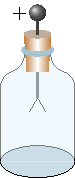
\includegraphics{fig/B/6-1a.pdf}
		\caption{}\label{fig_B_6-1a}
	\end{subfigure}
	\hfil
	\begin{subfigure}{0.3\linewidth}
		\centering
		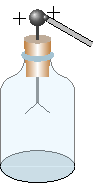
\includegraphics{fig/B/6-1b.pdf}
		\caption{}\label{fig_B_6-1b}
	\end{subfigure}
	\hfil
	\begin{subfigure}{0.3\linewidth}
		\centering
		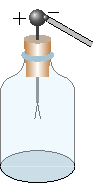
\includegraphics{fig/B/6-1c.pdf}
		\caption{}\label{fig_B_6-1c}
	\end{subfigure}
	\caption{}\label{fig_B_6-1}
\end{figure}



等量的异种电荷完全相互抵消的现象叫做中和.我们知道,物体是由原子组成的,原子是由带正电的原子核和带负电的电子组成的.
在通常的情况下,原子核所带的正电荷的电量(绝对值)等子所有电子所带负电荷的电量的总和(绝对值),原子呈中性状态,物体也呈中性状态,即对外表现为不带电的状态.
任何不带电的物体,其中都有等量的正负电荷,因而处于中性状态.

使物体带电叫做起电.起电的过程,实际上是使物体中的正负电荷分开的过程.在摩擦起电中,其中一个物体因失去一些电子而带正电,同时另一个物体因得到这些电子而带等量的负电.
摩擦起电并不是创造了电荷,只是电荷从一个
物体转移到另一个物体.

\subsection{静电感应} 

还有一种常见的使物体带电的方法叫感应起电.
取一对用绝缘柱支持的金属导体$A$和$B$,导体上都贴有金属箔,让$A$和$B$彼此接触,这时$A$和$B$上的金属箔闭合,表示它们都没有带电.把另一个带正电的金属球$C$移近导体$A$(图~\ref{fig_B_6-2a}),这时$A$、$B$上的金属箔都张开了,表示它们都带了电.实验表明,靠近$C$的导体$A$带的电荷与$C$异号,远离$C$的导体$B$带的电荷与$C$同号.
这种现象叫做\textbf{静电感应}.如果
先把$A$和$B$分开,然后移去$C$,则发现$A$和$B$仍带有电荷(图~\ref{fig_B_6-2b}).如果再让$A$和$B$重新接触,它们就呈现不带电的状态.这说明:$A$和$B$分开后所带的异种电荷是等量的,重新接触后等量异种电荷相互抵消.利用静电感应使物体带电的方法叫做\textbf{感应起电}.


\begin{figure}[htbp]
	\centering
	\begin{subfigure}{0.4\linewidth}
		\centering
		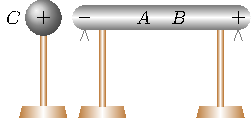
\includegraphics{fig/B/6-2a.pdf}
		\caption{}\label{fig_B_6-2a}
	\end{subfigure}
	\hfil
	\begin{subfigure}{0.4\linewidth}
		\centering
		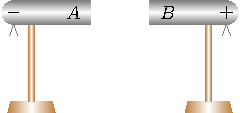
\includegraphics{fig/B/6-2b.pdf}
		\caption{}\label{fig_B_6-2b}
	\end{subfigure}
	\caption{静电感应}\label{fig_B_6-2}
\end{figure}




\subsection{电荷守恒定律} 

静电感应也是使物体中的电荷分开.
当我们把带正电的导体$C$移近绝缘导体时(图~\ref{fig_B_6-2a}),绝缘导体里的自由电子被吸引过来,因此导体两端分别带上等量异种电荷.可见,静电感应也不是创造了电荷,只是电荷从物体的一部分转移到另一部分.


大量事实说明:\textit{电荷既不能创造,也不能被消灭,它们只
能从一个物体转移到另一个物体,或者从物体的一部分转移到另一部分}.
这个结论叫做\textbf{电荷守恒定律}.它是物理学中重要的基本定律之一.

\subsection*{练习一}
\begin{enumerate}
\item 把支在绝缘座上的不带电的导体$A$移近带电体$B$,用手指接触一下$A$,然后移开手指,握住绝缘座移开导体$A$,导体$A$就带电了.如果带电体$B$原来带正电,导体$A$将带什么电?做这个实验并作出解释.
实验时可用验电器来检查导体$A$是否带电和带什么电.
\item 在图~\ref{fig_B_6-1} 中,先让验电器带上少量正电荷,然后拿一个带负电的带电体逐渐接近验电器的金属球,可以看到这
样的现象:金属箔张开的角度先是减小,以至闭合,然后又张开了.解释这个现象.
\end{enumerate}


\section{库仑定律}
\subsection{库仑定律} 

两个电荷间的相互作用力,跟它们的电量有关系,还跟电荷间的距离有关系.
法国物理学家库仑($1736 \sim 1806$)用实验研究了静止的点电荷间的相互作用力,于1785年发现了后来用他的名字命名的定律.

什么是点电荷呢?如果带电体间的距离比它们的大小大得多,以致带电体的形状和大小对相互作用力的影响可以忽略不计,这样的带电体就可以看成是点电荷.
跟力学中质点的概念类似,点电荷这个概念也是一种科学的抽象,是一种理
想化的模型.

\begin{figure}[htbp]
    \centering
    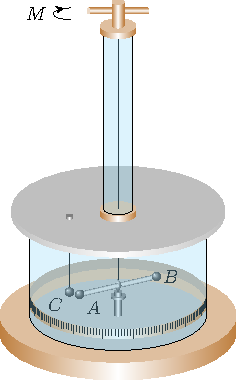
\includegraphics{fig/B/6-3.pdf}
    \caption{库仑扭秤}\label{fig_B_6-3}
\end{figure}

库仑是用图~\ref{fig_B_6-3} 所示的扭秤来做实验的.扭秤的主要部分是在一根细金属丝下面悬挂一根玻璃棒,棒的一端有一个
金属小球$A$,另一端有一个平衡小球$B$.
在离$A$球某一距离的地方再放一个同样的金属小球$C$,如果$A$球和$C$球带同种电荷,它们间的斥力将使玻璃棒转过一个角度.向相反方向扭转旋钮$M$,使玻璃棒回到原来的位置并保持静止,这时金属丝扭转弹力的力矩跟电荷间斥力的力矩平衡.因此从旋钮$M$转过的角度可以计算出电荷间作用力的大小.

库仑的实验是要研究电荷间的相互作用力跟它们间的距离和电量的关系.作用力跟距离的关系比较好办,保持两球的电量不变,改变两球的距离并测出作用力,就可以找出作用力跟距离的关系.困难在于作用力跟电量的关系,因为当时还不知道怎样测量电量,甚至连电量的单位也没有确定.库仑找到了一个简单办法巧妙地解决了这个问题.他把一个带电的金属球跟同样的但不带电的金属球相碰,两球带的电量一定相等,都是原有电量的$1/2$.同样可以得到原有电量的
$1/4$、$1/8$等等的电量.这样就可以用扭秤来研究电荷间的作用力跟电量的关系了.
库仑实验是在空气中做的,其结果跟在真空中相差很小.
库仑实验的结果是:\textbf{在真空中两个点电荷间的作用力跟它们的电量的乘积成正比,跟它们间的距离的平方成反比,作用力的方向在它们的连线上}.
这就是\textbf{库仑定律}.电荷间的这种作用力叫做\textbf{静电力},又叫做\textbf{库仑力}.

如果用$Q_1$、$Q_2$表示两个点电荷的电量,用$r$表示它们间的距离,用$F$表示它们间的静电力,库仑定律就可以写成下面的公式:
\begin{equation}\label{eq_B-6-1}
F=k\frac{Q_1Q_2}{r^2}
\end{equation}
式中$k$是比例常量,叫\textbf{静电力恒量},它的数值和单位由式中各量的单位决定.

我们很容易看出,库仓定律和万有引力定律很相似,它们都是平方反比定律.
人们现在还不能说明为什么这两个定律如此相似,但这种相似使我们可以用力学的比喻来理解许多电学问题,给我们的学习带来不少方便.

\subsection{电介质中的库仑定律} 

所谓电介质,就是我们在初中学过的绝缘体.空气、煤油、水、玻璃、橡胶、瓷器等都是电介质.

如果把两个电荷放在电介质里,例如放在煤油里,电荷间的作用力就比在同样情形下在真空里的作用力小.
小多少,依电介质的不同而不同.这时库仑定律用下面公式来表示:
\begin{equation}\label{eq_B-6-2}
F=k\frac{Q_1Q_2}{\varepsilon r^2}
\end{equation}

每一种电介质的$\varepsilon$的数值是一定的,叫做那种物质的\textbf{介电常数}.
表~\ref{tab_B_6-1} 是几种电介质的介电常数.实用上,通常把空
气的介电常数取为1,即认为电荷间的作用力在空气中跟在真空中一样.

\begin{table}[htbp]
	\centering
	\caption{}\label{tab_B_6-1}
    \begin{tblr}{c|ccccccc}
	\toprule
	电介质 & 空气&煤油&石蜡&陶瓷&玻璃&云母&水\\
	\midrule
	介电常数 & $1.0005$&$2$&$2.0 \sim 2.1$&6&$4 \sim 11$&$6 \sim 8$&$81$\\
	\bottomrule
    \end{tblr}
\end{table}

\subsection{电量的单位} 
在国际单位制中,电量的单位就是我们在初中学过的\textbf{库仑},简称库,国际符号是$\UCA$.

采用国际单位制,在库仑定律的公式中,力的单位用牛,距离的单位用米,电量的单位用库,各个量的单位都已经分别确定,这时静电力恒量的数值要由实验来确定.
实验指出:公式中的静电力恒量$k=9.0\times 10^9 \UNmqCq $.

\begin{example}
比较电子和质子间的静电引力和万有引力.
已知电子质量是$0.91\times 10^{-30}$千克,质子质量是$1.67\times 10^{-27}$
千克.
电子和质子的电量都是$1.60\times10^{-19}$
库.
\end{example}

    
\begin{solution}
电子和质子间的静电引力$F_{\text{电}}$和万有引力$F_{\text{引}}$分别是
\[F_{\text{电}} =k\frac{Q_1Q_2}{r^2} ,\qquad   F_{\text{引}}=G\frac{m_1m_2}{r^2} \]
因此,
\[\frac{F_{\text{电}}}{F_{\text{引}}}=\frac{kQ_1Q_2}{Gm_1m_2} \]

上式中$m_1$、$m_2$和$Q_1$、$Q_2$已知,$k=9.0\times 10^9 \UNmqCq$,
$G=6.67\times10^{-11} \UNmqkgq $.把数值代入进行计算,得
\[\begin{split}
    \frac{F_{\text{电}}}{F_{\text{引}}}&=\frac{9.0\times 10^9\times1.60\times10^{-19}\times1.60\times10^{-19}}{6.67\times10^{-11}\times 1.67\times10^{-27}\times 0.91\times10^{-30}}\\
    &=2.3\times 10^{39}
\end{split}\]
\end{solution}


从这个例题可以看出,电子和质子间的万有引力比它们
的静电引力小得多.正是因为这个缘故,在研究微观带电粒
子间的(如原子中电子和原子核间的)相互作用时,经常把万
有引力忽略不计.



\subsection*{练习二}

\begin{enumerate}
    \item 1库仑的电量是电子所带电量的多少倍?
    \item 在真空中有两个点电荷,电量分别为$+4.0\times10^{-9}$库
和$-2.0\times10^{-9}$库,相距10厘米.
这两个点电荷间的作用力
是多大?用电荷的绝对值代入进行计算,求出力的大小,然后
根据电荷的正负确定是引力还是斥力.
\item 在真空中有两个点电荷,保持它们的距离不变,它们
间的相互作用力在下列情况下将如何变化?
\begin{enumerate}
    \item 一个电荷的电量变为原来的2倍;
    \item 两个电荷的电量都变为原来的1/2.
\end{enumerate}
\item 原子核的半径大约为$10^{-14}$米,假定核中两个质子相距这么远,其间的静电力大约有多大?
\item 两个带电小球在煤油中相距0.5米.
其中一个小球
带电$5.0\times10^{-9}$库,另一个带电$3.0\times10^{-9}$库.
求小球间的作用力.
\item 当两个点电荷相距为$r$时,它们间的斥力为$F$.改
变电荷间的距离,当斥力为$16F$时,相距为多少?当斥力为
$\dfrac{1}{4}F$时,相距为多少?
\end{enumerate}


\section{电场~~电场强度}

\subsection{电场}
电荷间的相互作用是怎样发生的呢?

经过长期的科学研究,人们认识到:电荷之间的相互作用
是通过电场发生的.
只要有电荷存在,电荷周围就存在着电
场;电场的基本性质是它对放入其中的电荷有力的作用,这种力叫做电场力.
两个电荷$A$和$B$,电荷$A$受到的电荷$B$的作用,
实际上是电荷$B$的电场对电荷$A$的作用.同样,电荷$B$受到的
电荷$A$的作用,实际上是电荷$A$的电场对电荷$B$的作用.

历史上人们对场的认识是逐步深入的,我们理解场这个
概念也要有个过程,要逐步体会它的意义.引入场这个概念,
是对物理学的重要贡献.场的概念引入物理学之后取得了巨
大的成果.
除了电场,我们在初中还学过磁场,电场和磁场是
有联系的,常常总称为电磁场.
关于电磁场的研究导致了发现
电磁波.我们大家都熟悉的广播和电视就是借电磁波来传播
的.
电磁波可以脱离电荷而独立存在并以光速传播,它跟由
原子、分子组成的物质一样具有能量和动量.这样,人们逐渐
认识到:电磁场包括电场和磁场是物质的一种特殊形态.

电场这种物质跟由分子、原子组成的物质不同,看不见,
摸不到,好像不好理解.其实,电场跟其他物质一样,都是不
依赖于我们的感觉而客观存在的东西.在一位现代物理学家
看来,电场正像他所坐的椅子一样是客观存在.电场是在跟
电荷的相互作用中表现出自己的特性的.我们从电场所表现
出来的特性出发,加以分析研究,就可以懂得电场,认识
电场.

\subsection{电场强度} 

刚刚说过,电场的基本性质是它对放入其中
的电荷有电场力的作用.
现在来分析研究这个问题.

要研究电场,必须在电场中放入电荷.
而这个电荷应该
是一个电量很小的点电荷.电量很小,是为了使它放入之后,
不致影响原来要研究的电场.体积很小,是为了便于用它来
研究电场各点的性质.这样的电荷常常叫做检验电荷.


如图~\ref{fig_B_6-4} 所示,电场是由正电荷$Q$产生的,用挂在丝线下
端的带正电的小球作检验电荷,把它先后放在电场中不同的
位置,观察它在电场中的受力情况,力的大小可以从丝线对竖
直线偏角的大小看出.实验表明,检验电荷在电场中的位置
不同,受到的电场力的大小和方向也不同.检验电荷受到的
电场力大,说明那点的电场强;检验电荷受到的电场力小,说
明那点的电场弱.图~\ref{fig_B_6-4b} 中$A$点的电场强,$B$点的电场弱,
$C$点更弱.


\begin{figure}[htbp]
	\centering
	\begin{subfigure}{0.4\linewidth}
		\centering
		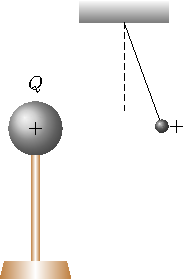
\includegraphics{fig/B/6-4a.pdf}
		\caption{}\label{fig_B_6-4a}
	\end{subfigure}
	\hfil
	\begin{subfigure}{0.4\linewidth}
		\centering
		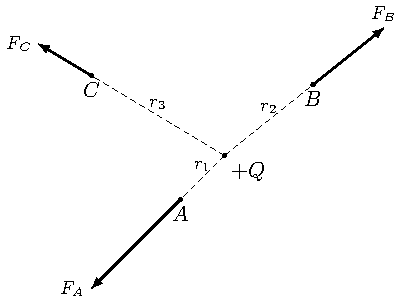
\includegraphics{fig/B/6-4b.pdf}
		\caption{}\label{fig_B_6-4b}
	\end{subfigure}
	\caption{}\label{fig_B_6-4}
\end{figure}



物理学中怎样来表示电场的强弱呢?把检验正电荷$q$放
到电场中的$A$点,电荷$q$受到电场力$F_A$的作用(图~\ref{fig_B_6-4b}).设
$A$点跟$Q$的距离为$r_1$,从库仑定律知道$F_A=kQq/r^2_1$.同样,如
果把正电荷$q'$放入$A$点,$q'$受到的电场力$F'_A=kQq'/r_1^2$.可
以看出,
\[\frac{F_A}{q}=\frac{F'_A}{q'}=\frac{kQ}{r^2_1} \]
这就是说,放入$A$点的电荷受到的电场力跟它的电量的比值,
是一个跟放入该点的电荷无关的恒量.

如果把电荷放入电场中的$B$点和$C$点,设$B$、$C$跟$Q$的距
离分别为$r_2$和$r_3$,同样可以证明,电荷在$B$和$C$受到的电场
力跟它的电量的比值分别是$kQ/r^2_2$、$kQ/r_3^2$,都是跟放入的电
荷无关的恒量.

可见,电荷在电场中某一点受到的电场力跟它的电量的
比值,由该点在电场中的位置所决定,跟放入的电荷无关.这
个比值越大的地方,放入那里的单位电荷受到的电场力越大,
电场就越强.这一点不仅对正电荷$Q$产生的电场是适用的,
对任何电场都是适用的.这就是说,对任何电场,都要用上述
比值来表示电场的强弱.

\textit{放入电场中某一点的电荷受到的电场力跟它的电量的比
值,叫做这一点的\textbf{电场强度}},简称为\textbf{场强}.跟力一样,电场强
度也是矢量,如果用$E$表示电场强度,用$F$表示检验电荷$q$受
到的电场力,那么
\begin{equation}\label{eq_B-6-3}
    E=\frac{F}{q}
\end{equation}

由~\eqref{eq_B-6-3} 式可以知道,如果$q$为单位正电荷,那么$E$和$F$在
数值上相等,可见电场中某一点的场强在数值上等于单位正
电荷在那一点所受的电场力.正负电荷在电场中某点所受电
场力的方向相反.
我们规定场强的方向是正电荷受力的方向.
这样,负电荷受力的方向跟场强的方向相反.

场强的单位是牛/库($\UNCA$).电场中的某一点,如果1库的点电
荷在该点受到的电场力是1牛,这点的场强就是1$\UNC$.

从上面讲的很容易知道,点电荷$Q$在真空中形成的电场
中,在距离$Q$为$r$的$P$点的场强$E$的大小为
\begin{equation}\label{eq_B-6-4}
    E=\frac{kQ}{r^2}
\end{equation}

这个公式只适用于真空,如果在充满电介质的空间里,这
个公式应改写成
\begin{equation}\label{eq_B-6-5}
    E=\frac{kQ}{\varepsilon r^2}
\end{equation}

如果$Q$是正电荷,$E$的方
向就背离$Q$;如果$Q$是负电荷,
$E$的方向就指向$Q$(图~\ref{fig_B_6-5}).
\begin{figure}[htbp]
    \centering
    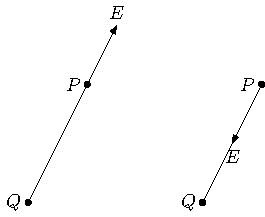
\includegraphics{fig/B/6-5.pdf}
    \caption{场强的方向}\label{fig_B_6-5}
\end{figure}

应该注意,\eqref{eq_B-6-3} 式、\eqref{eq_B-6-4} 式和~\eqref{eq_B-6-5} 式虽然都表示电场中某点
的场强,但它们的意义是不同
的.\eqref{eq_B-6-3} 式是场强的定义式,对任何电场都适用.\eqref{eq_B-6-4} 式是点电荷在真空中各点场强的计算
式,只适用于点电荷在真空中的电场.\eqref{eq_B-6-5} 式是点电荷在充满
电介质空间里各点场强的计算式.

如果有几个点电荷同时存在,它们的电场就互相叠加,形
成合电场.
这时某点的场强,就等于各个点电荷在该点产生
的场强的矢量和.这样,知道了点电荷的场强,原则上我们就
可以知道任一带电体的场强,因为任何带电体都可以看作是
由许多点电荷组成的.

\section*{阅读材料:用比值定义物理量}
在物理学中,常常用比值来定义一个物理量.

我们在初中学过密度.
在那里我们学到:单位体积的某
种物质的质量,叫做这种物质的密度.其实,密度也可以用比值来定义.
某种物质的物体,它的质量与它的体积成正比.因
此我们可以这样表达密度的定义:某种物质组成的物体,它的
质量和它的体积的比值,叫做这种物质的密度.
对某种物质来说,这个比值是恒定的;对不同的物质来说,这个比值一般并不相同.
因此,密度表示物质的一种特性.

初中学过的电阻是用比值来定义的.一段导体中的电流
强度跟加在这段导体上的电压成正比.
导体两端的电压跟通
过导体的电流强度的比值,叫做这段导体的电阻.当温度保
持不变时,对某段导体来说,这个比值是恒定的;对不同的导
体来说,这个比值一般并不相同.这个比值越大,表示导体对
电流的阻碍作用越大.因此,电阻是表示导体对电流阻碍作
用的物理量.

刚刚学过的电场强度也是用比值来定义的.放入电场中
某点的电荷受到的电场力跟它的电量成正比.放入电场中某
点的电荷受到的电场力跟它的电量的比值,叫做这一点的电
场强度.对电场中的某一点,这个比值是恒定的;对电场中的
不同的点,这个比值一般并不相同.这个比值越大,表示那一
点的电场越强.电场强度是表示电场的力的性质的物理量.

不再一一列举.我们看到这里有一个共同点,那就是要
在实验的基础上寻求一个只与所研究的物体或场有关的比
值,来表示物体或场的某种性质,并由这个比值定义一个新
的物理量.在定义这个新的物理量的同时,也就确定了这个
新的物理量与已有物理量之间的关系.例如,定义了密度,
也就确定了密度、体积和质量这三者的关系.这里我们一定
要注意到这个比值是反映物体或场的什么性质,这样才能很
好地理解它的物理意义.

在今后的学习中,还会遇到用比值来定义的物理量.因
此,我们要很好地体会这种定义物理量的方法.

\subsection*{练习三}

\begin{enumerate}
    \item 在正电荷$Q$的电场中的某一点放一个电荷,它的电
    量$q=10^{-8}$库,$q$受到的电场力为$10^{-8}$牛.求这一点的电场
    强度$E$,并指出电场强度的方向.如果取走$q$,$E$有无变化?
    为什么?
    \item 在以水为介质的负点电荷$Q$的电场中,离$Q$在0.5米处
    的电场强度$E$是1$\UNC$,求负电荷Q的电量是多少库.
    \item 电场中某点的场强是$0.2\times10^5\UNC$.求电量为
    $2\times10^{-8}$库的正电荷在该点受到的电场力是多大.
    \item 在氢原子中,电子和质子的平均距离是$5.3\times10^{-11}$
    米.质子在这个距离处产生的场强是多大?方向如何?电子
    受到的力是多大?方向如何?
    \item 物理学上常把重力作用的空间叫做\textbf{重力场}.如果把
    单位质量的物体受到的重力叫做重力场强度,试写出重力场
    强度的定义式.重力场强度的方向如何?从重力场强度的方
    向来看,重力场是跟正电荷形成的电场相似,还是跟负电荷形
成的电场相似?
\item 电场强度的定义式$E=F/q$在电介质中要不要改
写?为什么?
\end{enumerate}


\section{电力线}
\subsection{电力线}

研究电场,重要的是要知道电场中各点场强的
大小和方向.如果能够用图形把电场中各点场强的大小和方
向形象地表示出来,这对我们认识电场是很有好处的.图~\ref{fig_B_6-6} 
是在正电荷和负电荷的电场中画出的一组矢量,表示出场内
一些点的场强的大小和方向.但是,更好的办法是用英国物
理学家法拉第($1791 \sim 1867$)引入的电力线来形象地表示
电场.
\begin{figure}[htbp]
    \centering
    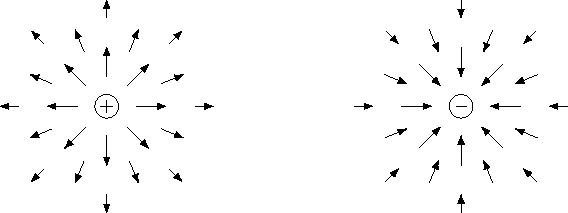
\includegraphics{fig/B/6-6.pdf}
    \caption{}\label{fig_B_6-6}
\end{figure}

在任何电场中,每一点的场强$E$都有一定的方向,所以
我们可以在电场中画出一系列的从正电荷出发到负电荷终止
的曲线,使曲线上每一点的切线方向都跟该点的场强方向一
致,这些曲线就叫做\textbf{电力线}.图~\ref{fig_B_6-7} 是一条电力线,它上面的
$A$、$B$点的场强$E_A$、$E_B$在各该点的切线上,方向如图中箭头
所示.
\begin{figure}[htbp]
    \centering
    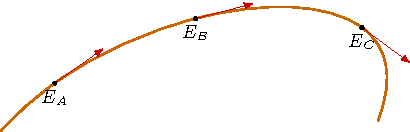
\includegraphics{fig/B/6-7.pdf}
    \caption{}\label{fig_B_6-7}
\end{figure}

电力线的形状可以用实验来观察.把奎宁的针状结晶、
木屑或头发屑悬浮在蓖麻油里,再放入电场中,就可以看到微
屑按照场强的方向排列起来(图~\ref{fig_B_6-8}),显示出电力线的形状.
应该注意,虽然我们可以用实验来显示电力线的形状,但电力
线并不是电场里实际存在的线,而是人们为了使电场形象化
而假想的线.
\begin{figure}[htbp]\centering
    \begin{subfigure}{0.4\linewidth}
        \centering
        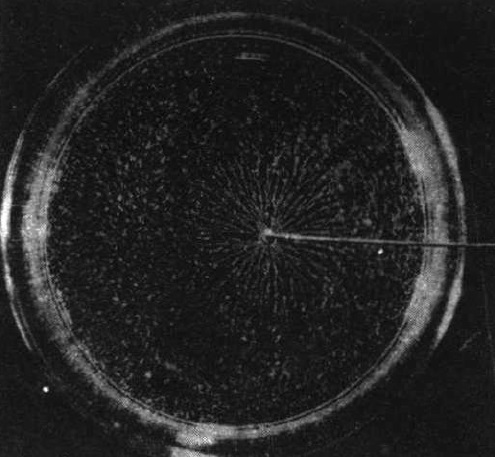
\includegraphics[height=4cm]{fig/B/6-8a.jpg}
        \caption{点电荷的电力线形状}\label{fig_B_6-8a}
    \end{subfigure}
    \hfil
    \begin{subfigure}{0.4\linewidth}
        \centering
        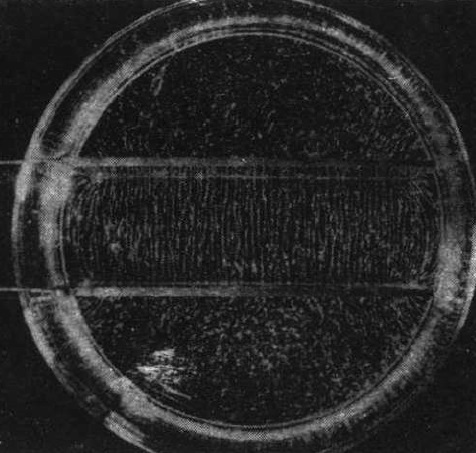
\includegraphics[height=4cm]{fig/B/6-8b.jpg}
        \caption{带相反电荷的平行板间的电力线形状}\label{fig_B_6-8b}
    \end{subfigure}
    \caption{}\label{fig_B_6-8}
\end{figure}

    
图~\ref{fig_B_6-9} 是点电荷的电力线,图~\ref{fig_B_6-10} 是两个等量的电荷的
电力线.从图中可以看出,在离形成电场的电荷越近的地方,
也就是场强越大的地方,电力线越密.所以,用电力线不但可
以形象地表示电场强度的方向,还可以表示电场强度的大小:
场强越大的地方电力线越密,场强越小的地方电力线越稀.


\begin{figure}[htbp]
	\centering
	\begin{subfigure}{0.4\linewidth}
		\centering
		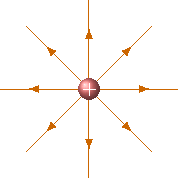
\includegraphics{fig/B/6-9a.pdf}
		\caption{正电荷}\label{fig_B_6-9a}
	\end{subfigure}
	\hfil
	\begin{subfigure}{0.4\linewidth}
		\centering
		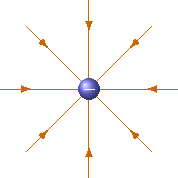
\includegraphics{fig/B/6-9b.pdf}
		\caption{负电荷}\label{fig_B_6-9b}
	\end{subfigure}
	\caption{点电荷的电力线}\label{fig_B_6-9}
\end{figure}


\begin{figure}[htbp]
    \centering
    \begin{subfigure}{0.4\linewidth}
        \centering
        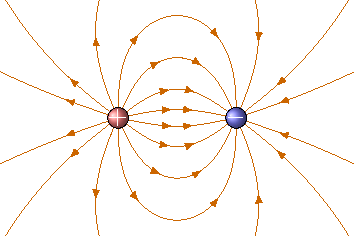
\includegraphics{fig/B/6-10a.pdf}
        \caption{等量异种电荷}\label{fig_B_6-10a}
    \end{subfigure}
    \hfil
    \begin{subfigure}{0.4\linewidth}
        \centering
        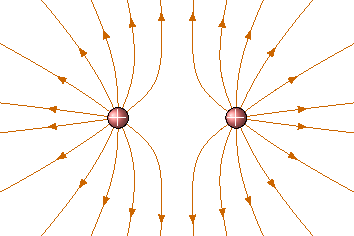
\includegraphics{fig/B/6-10b.pdf}
        \caption{等量同种电荷}\label{fig_B_6-10b}
    \end{subfigure}
    \caption{两个等量电荷的电力线}\label{fig_B_6-10}
\end{figure}
    


\subsection{匀强电场} 

在电场的某一区域里,如果各点的场强的大
小和方向都相同,这个区域的电场就叫做\textbf{匀强电场}.匀强电
场是最简单的同时也是很重要的电场,在实验研究中常常要
用到它.

在匀强电场里,既然各点的场强的方向都相同,电力线就
一定是互相平行的直线;既然各点的场强的大小都相同,电力
线的疏密程度也一定处处相等.因此,匀强电场中的电力线
是距离相等的互相平行的直线.

两块靠近的平行金属板,
它们的大小相等并且互相正
对,在分别带等量的正电和负
电的时候,它们之间的电场,除
边缘附近外,就是匀强电场(图~\ref{fig_B_6-11}).

\begin{figure}[htbp]
    \centering
    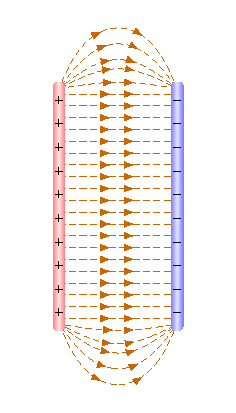
\includegraphics{fig/B/6-11.pdf}
    \caption{匀强电场}\label{fig_B_6-11}
\end{figure}

\section*{阅读材料:法拉第和场的概念}
相隔一定距离的电荷或磁体间的相互作用是怎样发生
的,这个问题在历史上有过长期的争论.十九世纪前期,大部
分物理学家认为电荷或磁体间的相互作用是超距作用.所谓
超距作用是指这种作用不需要任何媒质传递,就能够由一个
物体立即作用到另一个物体.

然而法拉第通过实验发现,电作用或磁作用跟电荷之间
或磁体之间的媒质有关.他在不同的媒质中进行同样的实验,
其作用效果不同.这引起他对电磁作用本质的深思.法拉第
认为,电磁力不可能是超越空间并与空间中媒质无关的超距
作用.法拉第提出了关于电磁作用的新看法:电荷或磁体在
周围空间产生电场或磁场,正是通过场,才把电作用或磁作用
传递到别的电荷或磁体.

经典力学是以超距作用为基础的.
空间中除了粒子以外
什么也没有,没有粒子的地方是一无所有的真空;粒子间的相
互作用是超距作用,不需要通过媒质传递.法拉第提出的场
的模型从基本概念上突破了经典力学的框架,为建立近代物
理开创了新的起点.

法拉第凭着敏锐的直觉不仅提出了场的概念,而且描绘
出一幅清晰的场的图像.他用电力线或磁力线形象地表示电
场和磁场.
力线密的地方场就强,力线疏的地方场就弱.力线
上每一点的切线方向表示场强的方向.
法拉第用这幅图像解
释了用经典力学无法解释的现象.
例如,1831年他发现了电磁
感应现象,他借助于磁力线对这一现象很快地作出了解释:只
要通过闭合电路的磁力线数目发生变化,电路里就会产生
电流.

法拉第提出的场的概念还处于萌芽状态.后来麦克斯韦
用数学方程定量地描述了电磁场的定律,预言了电磁波的存
在,并且把光现象和电磁现象联系起来,得出光波是一种电磁
波的结论.场的概念取得了很大成功,并逐渐在物理学中取
得了主要地位,是基本的物理概念之一.

\subsection*{练习四}

\begin{enumerate}
    \item 有人说电力线就是带电粒子在电场中运动的轨迹.这种说法对吗?为什么?
    \item 在图~\ref{fig_B_6-9} 到图~\ref{fig_B_6-11} 中,所有的电力线都不相交.
    我们能否断言,电场中任何两条电力线都不相交.
    为什么?
\end{enumerate}

\section{电场中的导体}
我们在初中学过,导体的特征是它的内部有大量的可以
移动的自由电荷.对于金属导体来说,这种自由电荷就是自
由电子.金属原子的最外层电子跟原子核的联系很弱,在其
余原子的作用下会脱离原来的原子而在整块金属中自由“游
荡”,成为自由电子.失去了外层电子的原子变成带正电的离
子,在平衡位置附近做热振动.所以,整块金属就是由做热振
动的正离子和在它们之间做无规则的热运动的自由电子组
成的.

\subsection{静电平衡状态} 


把一个不带电的金属导体$ABCD$放到场
强为$E_0$的电场中,导体内部的自由电子受到电场力的作用,
将向电场的反方向做定向移动(图~\ref{fig_B_6-12a}).这样,在金属的
$AB$面上将出现负电荷,在$CD$面上将出现正电荷.
这种导体里的自由电荷由于受到外电场的作用而重新分布的现象,就
是我们前面讲过的静电感应.导体两端出现的正负电荷在导
体内部形成反方向的电场$E'$,它的电力线用虚线表示(图~\ref{fig_B_6-12b}).
这个电场与外电场叠加,使导体内部的场强减小.但
是,只要导体内部的场强不等于零,自由电子就继续移动,两
端的正负电荷就继续增加,导体内部的电场就进一步削弱,直
到导体内部各点的场强都等于零时为止.这时自由电子的定
向移动停止(图~\ref{fig_B_6-12c}).

\begin{figure}[htbp]
	\centering
	\begin{subfigure}{0.32\linewidth}
		\centering
		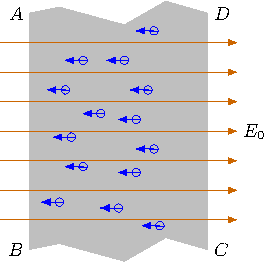
\includegraphics{fig/B/6-12a.pdf}
		\caption{}\label{fig_B_6-12a}
	\end{subfigure}
	\hfil
	\begin{subfigure}{0.32\linewidth}
		\centering
		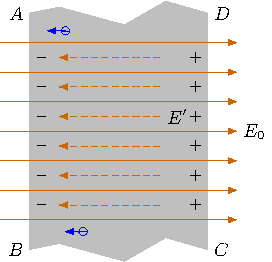
\includegraphics{fig/B/6-12b.pdf}
		\caption{}\label{fig_B_6-12b}
	\end{subfigure}
	\hfil
	\begin{subfigure}{0.32\linewidth}
		\centering
		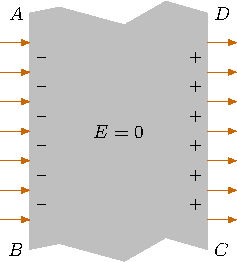
\includegraphics{fig/B/6-12c.pdf}
		\caption{}\label{fig_B_6-12c}
	\end{subfigure}
	\caption{}\label{fig_B_6-12}
\end{figure}


导体中(包括表面)没有电荷定向移动的状态叫做\textbf{静电平
衡状态}.\textit{处于静电平衡状态的导体,内部的场强处处为零}.

导体处于静电平衡状态时,它表面的场强方向一定跟它
的表面垂直(参看图~\ref{fig_B_6-12c}).假如不是这样,场强就有一个
沿导体表面的分量,导体上的自由电子就会发生定向移动,这就不是平衡状态了.
所以,\textit{处于静电平衡状态的导体,表面上
任何一点的场强方向跟该点的表面垂直}.

带电导体可以认为它处于本身所带电荷形成的电场中,
它在静电平衡状态时内部的场强也一定处处为零.
假如不是这样,导体内部的自由电子就会发生定向移动.
既然导体内
部的场强处处为零,导体内部就不可能有未被抵消的电荷.这
是因为,假如在导体内部某处有电荷,在它的附近的场强就不可能为零.
所以,\textit{处于静电平衡状态的带电导体,电荷只能分
布在导体的外表面上}.

静电平衡时电荷只分布在导体的外表面上,可以用下述
的法拉第圆筒实验来验证.如图~\ref{fig_B_6-13} 所示,取两个验电器$A$
和$B$,在$B$上装一个几乎封闭的空心金属圆筒$C$(叫做法拉第
圆筒).使$B$和$C$带电,$B$的箔片张开.
用有绝缘柄的金属小
球$e$先跟$C$的外部接触,再把$e$移到$A$并跟$A$的金属球接触
(图~\ref{fig_B_6-13}).经过若干次以后,可以看到$A$的箔片张开,同时
$B$的箔片张开的角度减小.这表明$e$把$C$的一部分电荷搬运
给了$A$.可见法拉第圆筒的外表面是带有电荷的.如果让$e$
不接触$C$的外部,而接触$C$的内部,重做上述实验(图~\ref{fig_B_6-14}),
不论重复多少次,$A$的箔片都不张开,$B$的箔片张开的角度也不减小.
这表明$e$并没有把$C$的电荷搬运给$A$,可见拉法第
圆筒的内部不带电.

\begin{figure}[htbp]
    \centering
    \begin{minipage}[t]{0.48\textwidth}
    \centering
    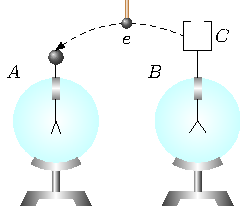
\includegraphics{fig/B/6-13.pdf}
    \caption{}\label{fig_B_6-13}
    \end{minipage}
    \begin{minipage}[t]{0.48\textwidth}
    \centering
    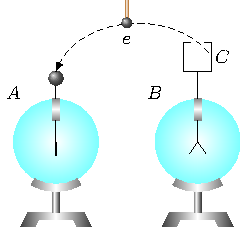
\includegraphics{fig/B/6-14.pdf}
    \caption{}\label{fig_B_6-14}
    \end{minipage}
\end{figure}

\subsection{静电屏蔽}

静电平衡时导体内部的场强为零这一现象,
在技术上用来实现静电屏蔽.


如图~\ref{fig_B_6-15a} 所示,使带正电的金属球靠近验电器,由于
静电感应,验电器的箔片张开,这表示验电器受到了附近的带
电体的影响.如果事先用一个金属网罩把验电器罩住(图~\ref{fig_B_6-15b}),
再让带电金属球靠近,验电器的箔片就不张开了.即使
用导线把验电器和金属网罩连接上,箔片也不张开.可见,金
属网罩(或金属包皮)能把外电场遮住,使内部不受外电场的
影响,这就是\textbf{静电屏蔽}.有的电学仪器和电子设备的外面套
有金属罩,通讯电缆的外面包一层铅皮,都是用来防止外界
电场的干扰起屏蔽作用.

\begin{figure}[htbp]
    \centering
    \begin{subfigure}{0.4\linewidth}
        \centering
        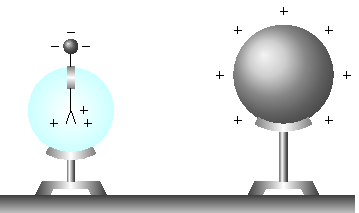
\includegraphics{fig/B/6-15a.pdf}
        \caption{}\label{fig_B_6-15a}
    \end{subfigure}
    \hfil
    \begin{subfigure}{0.4\linewidth}
        \centering
        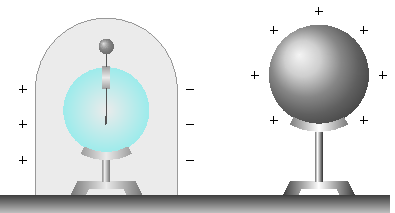
\includegraphics{fig/B/6-15b.pdf}
        \caption{}\label{fig_B_6-15b}
    \end{subfigure}
    \caption{静电屏蔽}\label{fig_B_6-15}
\end{figure}


\section{电势能}
前面我们从电荷在电场中受到力的作用出发,研究了电
场的性质.
下面我们从能量的角度来研究电场的性质.

我们知道,物体在重力场中具有重力势能.
重力势能是与重力做功密切相关的.
同样,电荷在电场中也具有势能,叫
做电势能.电势能是与电场力做功密切相关的.

物体在地面附近下落时,重力对物体做正功,重力势能减
少;物体上升时,重力对物体做负功,重力势能增加.
重力势能的变化总等于重力对物体所做的功.与此相似,在电场中
移动电荷时,如果电场力对电荷做正功,电势能就减少;如果
电场力对电荷做负功,电势能就增加.电势能的变化总等于
电场力对电荷所做的功.

就功和能之间的关系来讲,电场中的情形跟重力场中的
情形完全相似.但由于存在两种电荷,电场力既可以是引力,
也可以是斥力,因此电场力做功的问题要复杂一些.

图~\ref{fig_B_6-16} 表示正电荷$Q$的电场,在电场中把正电荷$q$从$A$
点移到$B$点,电场力的方向与电荷移动的方向相同,电场力对
电荷$q$做正功,电势能减少.可见,正电荷$q$在$A$点的电势能
大于它在$B$点的电势能.在正电荷$Q$的电场中,正电荷$q$离
$Q$越近,电势能越大.
\begin{figure}[htbp]
    \centering
    \begin{minipage}[t]{0.48\textwidth}
        \centering
        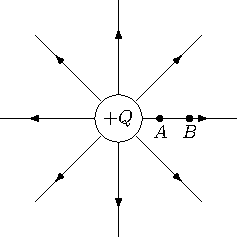
\includegraphics{fig/B/6-16.pdf}
        \caption{正电荷$Q$的电场}\label{fig_B_6-16}
    \end{minipage}
    \begin{minipage}[t]{0.48\textwidth}
        \centering
        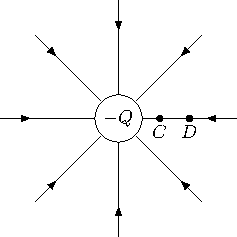
\includegraphics{fig/B/6-17.pdf}
        \caption{负电荷$Q$的电场}\label{fig_B_6-17}
    \end{minipage}
\end{figure}

图~\ref{fig_B_6-17} 表示负电荷$Q$的电场,在电场中把正电荷$q$从$C$
点移到$D$点,电场力的方向与电荷移动的方向相反,电场力对
电荷$q$做负功,电势能增加.可见,正电荷$q$在$C$点的电势能
小于它在$D$点的电势能.在负电荷$Q$的电场中,正电荷$q$离
$Q$越近,电势能越小.

我们在讨论重力势能的时候,要先规定物体在某一位置
的重力势能为零,然后才能确定物体在其他位置的重力势能.
物体在某一位置的重力势能在数值上等于物体从这一位置移
到重力势能为零处重力所做的功.同样,我们在讨论电势能
的时候,也要先规定电荷在某一位置的电势能为零,然后才能
确定电荷在其他位置的电势能.\textit{电荷在电场中某点的电势能
在数值上等于把电荷从这点移到电势能为零处电场力所做的
功}.

在理论研究中,通常取电荷$q$在无限远处的电势能为零.
这样,在图~\ref{fig_B_6-16} 所示正电荷的电场中,因为正电荷$q$在离开
$Q$越远的地方电势能越小,而它在无限远处的电势能为零,所
以正电荷$q$在正电荷$Q$的电场中的电势能都是正值.在图~\ref{fig_B_6-17} 
所示的负电荷的电场中,因为正电荷$q$在离开电荷$Q$越
远的地方电势能越大,而它在无限远处的电势能为零,所以正
电荷$q$在负电荷$Q$的电场中电势能都是负值.


\subsection*{练习五}

\begin{enumerate}
    \item 把两个异种电荷的距离增大一些,电场力做正功还
是做负功?电势能是增加还是减小?把两个同种电荷的距离增
大一些,情况又怎样?
\item 在图~\ref{fig_B_6-16} 中,把负电荷$-q$放在$A$、$B$点,它在哪一点
的电势能较大?无限远处的电势能为零,负电荷$-q$在这个
电场中的电势能是正值还是负值?
\item 在图~\ref{fig_B_6-17} 中,把负电荷$-q$放在$C$、$D$点,它在哪一点的电势能较大?取无限远处的电势能为零,负电荷$-q$在这
个电场中的电势能是正值还是负值?
\item 在图~\ref{fig_B_6-18} 所示的电场中,如果把正电荷$q$由$N$点移到$M$点,$q$的电势能增加还
是减小?如果移动的是负电荷$-q$,电势能又怎样变化?
\begin{figure}[htbp]
    \centering
    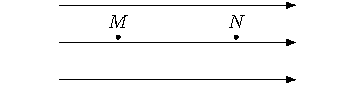
\includegraphics{fig/B/6-18.pdf}
    \caption{}\label{fig_B_6-18}
\end{figure}    

\item  电子在原子核附近运动时,电子的电势能是正值还
是负值?取无限远处的电势能为零.
把这个电子由原子核附
近移到无限远处,电子的电势能是增加还是减小?
\end{enumerate}


\section{电势}
电荷在电场中某点具有的电势能跟电荷所带的电量有关
系.设在图~\ref{fig_B_6-16} 所示的正电荷的电场中,正电荷$q$在$A$点的
电势能为$\mathcal{E}_A$,它在数值上等于把电荷$q$从$A$点移到无限远处电场力所做的功.
如果把放在$A$点的电荷增加为原来的$n$倍,
那么,在把它移到无限远处的过程中,所受的电场力处处为原
来的$n$倍,电场力所做的功也为原来的$n$倍,因而电势能为原
来的$n$倍.这就是说,电荷在电场中某点具有的电势能$\mathcal{E}_A$跟
电荷所带的电量$q$成正比,不论电量$q$是多少,比值$\mathcal{E}_A/q$都相
同,是跟电量$q$无关的一个恒量.

把正电荷$q$放在图~\ref{fig_B_6-16} 中的$B$点,设电荷的电势能为$\mathcal{E}_B$
.根据同样的分析知道,比值$\mathcal{E}_B/q$也是跟电量无关的
恒量.因为$\mathcal{E}_B$
跟$\mathcal{E}_A$一般并不相同,所以比值$\mathcal{E}_B/q$跟$\mathcal{E}_A/q$
一般也不相同.

上面是就正电荷$Q$产生的电场来分析的,实际上,上述分
析对任何电场都是适用的.

既然在电场中某点比值$\mathcal{E}/q$是跟电量$q$无关的恒量,而
且对电场中不同的点来说这个恒量一般并不相同,可见,这个
恒量是由电场本身决定的,它反映电场本身的一种性质.

\textit{电场中某点的电荷的电势能跟它的电量的比值,叫做这
一点的\textbf{电势}}.
如果用$U$表示电势,用$\mathcal{E}$表示电荷$q$的电势能,
那么
\[U=\frac{\mathcal{E}}{q} \]

如果取$q$为单位正电荷,那么$U$在数值上等于$\mathcal{E}$.可见,
电场中某点的电势在数值上等于单位正电荷在那一点所具有
的电势能.

在国际单位制中,电势的单位是伏特,简称伏,国际符号
是$\UVA$.电场中的某一点,如果电量是1库的电荷在该点的电
势能是1焦,这一点的电势就是1伏.
\[ 1 \UV =1 \UJC \]

电势只有大小,没有方向,因此是标量.

电势跟电势能一样,并没有绝对的意义.只有先规定了某
处的电势为零以后,才能确定电场中其他各点的电势的值.电
场中电势为零的位置也就是电荷在该点的电势能为零的位
置.在理论研究中,通常也就取无限远处的电势为零.在实
际应用中,通常取大地的电势为零.

在规定了零电势后,电场中各点的电势可以是正值,也可
以是负值.例如,规定无限远处的电势为零,在图~\ref{fig_B_6-16} 所示
的正电荷$Q$的电场中,因为正电荷$q$的电势能都是正值,所以
电场中各点的电势都是正值,而且离正电荷$Q$越远,电势越
低;在图~\ref{fig_B_6-17} 所示的负电荷$Q$的电场中,因为正电荷$q$的电
势能都是负值,所以电场中各点的电势都是负值,而且离负电
荷$Q$越远,电势越高.

在电场中,我们可以根据电力线的方向判断电场中各点
电势的高低.
因为顺着电力线的方向移动正电荷,电场力做
正功,正电荷的电势能减小,所以\textit{顺着电力线的方向电势越来
越低}.这个结果不但对正电荷或负电荷的电场是适用的,对
任何电场都适用.

现在我们已经认识了反映电场性质的两个物理量:电场
强度和电势.\textit{电场强度是反映电场的力的性质的物理量}.知
道了电场强度$E$,就可以知道电荷$q$在电场中所受的力$F=qE$.
\textit{电势是反映电场的能的性质的物理量}.知道了电势$U$,
就可以知道电荷$q$在电场中的电势能$\mathcal{E}=qU$.在电势为正值
的地方,正电荷的电势能是正值,负电荷的电势能是负值.在
电势为负值的地方,正电荷的电势能是负值,负电荷的电势能
是正值.

\section{等势面}

我们知道,用电力线能够把电场中各点场强的大小和方
向形象地表示出来.电场中各点电势的大小,是否也可以用
图形来表示呢?同样可以.
一般说来,电场中各点的电势不
同,但电场中有许多点的电势相等.我们把电场中电势相等
的点构成的面叫做\textbf{等势面}.在电场中可以用等势面来表示电
势的高低,这跟在地图上用等高线来表示地形的高低是类似
的.

在同一等势面上的任何两点间移动电荷,电场力不做功.
这是因为,假如电场力做了功,这两点的电势就不相等,它们
就不在一个等势面上了.这种情形,跟在同一水平面上的两
点间移动物体时,重力不做功的道理是一样的.

等势面一定跟电力线垂直,即跟场强的方向垂直.假如
不是这样,场强就有一个沿着等势面的分量,这样在等势面上
移动电荷时电场力就要做功.
但这是不可能的,因为在等势
面上各点电势相等,沿等势面移动电荷时电场力是不做功的.
所以场强一定跟等势面垂直.

前面已经指出,沿着电力线方向电势越来越低.可见,电
力线不但跟等势面垂直,而且是由电势较高的等势面指向电
势较低的等势面.




图~\ref{fig_B_6-19} 是匀强电场中的等势面,它们是垂直于电力线的
一族平面.图~\ref{fig_B_6-20} 是点电荷电场中的等势面,它们是以点电
荷为球心的一族球面.图~\ref{fig_B_6-21} 是等量异种的两个点电荷电
场中的等势面.

\begin{figure}[htbp]
	\centering
	\begin{minipage}[t]{0.48\textwidth}
		\centering
		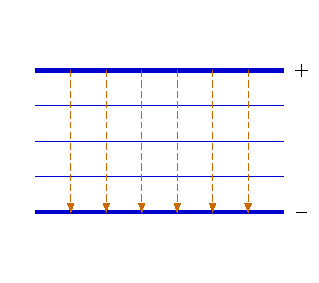
\includegraphics{fig/B/6-19.pdf}
		\caption{}\label{fig_B_6-19}
	\end{minipage}
	\begin{minipage}[t]{0.48\textwidth}
		\centering
		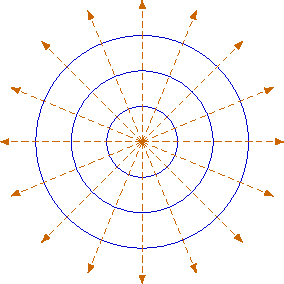
\includegraphics{fig/B/6-20.pdf}
		\caption{}\label{fig_B_6-20}
	\end{minipage}
\end{figure}



导体在静电平衡状态时内部场强处处为零,在导体的任
意两点间移动电荷时电场力所做的功等于零,因此导体内各
点的电势相等.\textit{处于静电平衡状态的导体是一个等势体,
它
的表面是一个等势面}.图~\ref{fig_B_6-22} 
是不规则形状的带电导体周
围的电力线和等势面的分布情
况.导体的表面是个等势面;
离导体表面越近,等势面的形
状与导体表面的形状越相似.

\begin{figure}[htbp]
	\centering
	\begin{minipage}[t]{0.46\textwidth}
		\centering
		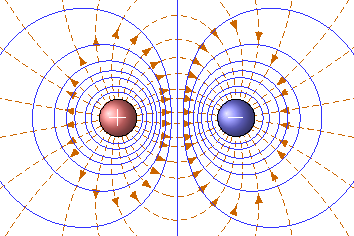
\includegraphics{fig/B/6-21.pdf}
		\caption{}\label{fig_B_6-21}
	\end{minipage}
	\begin{minipage}[t]{0.5\textwidth}
		\centering
		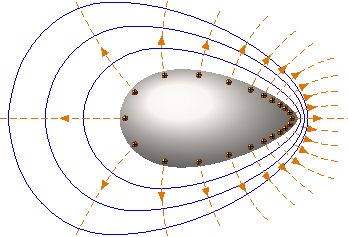
\includegraphics[scale=1.1]{fig/B/6-22.pdf}
		\caption{带电导体周围的等势面和电力线}\label{fig_B_6-22}
	\end{minipage}
\end{figure}



实际测量电势比测量场强容易,所以常常用等势面来研
究电场.
先测绘出等势面的形状和分布,再根据电力线和等势面
处处垂直这一特性,绘出电力线的形状和分布,就可以知
道整个电场的分布.设计许多电子仪器(如电子显微镜、示波
管等)中的电极的形状、大小及相互位置时,都需事先经过实
验,测绘出等势面的形状和分布,推知带电电极所产生的电场
的分布,以便找出符合实际要求的设计方案.


\subsection*{练习六}

\begin{enumerate}
    \item 电场中A点的电势是3伏.求:
    \begin{enumerate}
        \item 电量为5库的电荷在$A$点的电势能;
        \item 电量为10库的电荷在$A$点的电势能;
        \item 电量为$-5$库的电荷在$A$点的电势能;
        \item 电量为$-10$库的电荷在$A$点的电势能.
    \end{enumerate}
    \item 在图~\ref{fig_B_6-16} 中$A$、$B$两点哪一点电势高?在图~\ref{fig_B_6-17} 中
$C$、$D$两点哪一点的电势高?说明理由.

\item 在图~\ref{fig_B_6-23} 所示的匀强
电场中,如果$A$板是接地的,
$M$、$N$两点哪点电势高?电势是
正值还是负值?如果$B$板是接
地的,结果又怎样?取大地的电
势为零.

\begin{figure}[htbp]
    \centering
    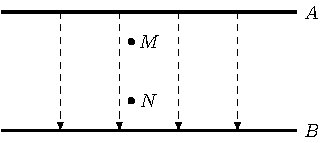
\includegraphics{fig/B/6-23.pdf}
    \caption{}\label{fig_B_6-23}
\end{figure}    

\item 一个初速度为零的正电荷放在电场中,只在电场力
作用下,它向电势高的地方跑还是向电势低的地方跑?一个初
速度为零的电子放在电场中,它向电势高的地方跑还是向电
势低的地方跑?说明理由.
\item 一个初速度为零的电荷放在电场中,不论是正电荷
还是负电荷,都向着电势能低的地方跑.
试说明理由.
\item 电场中某点的电势是否跟检验电荷的正负有关?讨
论一下这个问题.
\item 电场中两个电势不同的等势面能不能相交?为什么?
\end{enumerate}

\section{电势差}
用不同的位置作为测量高度的起点,同一地方的高度的
数值就不相同,但两个地方的高度差保持不变.
同样的道理,
选择不同的位置作零电势,电场中某点的电势的数值也会改
变,但电场中任意两点间的电势的差值保持不变.
正是因为这
个缘故,在物理学中电势的差值用得比电势更为普遍.

\subsection{电势差}
\textit{电场中两点间的电势的差值叫做\textbf{电势差},有时又叫做\textbf{电压}}.
设电场中$A$点的电势为$U_A$,$B$点的电势为$U_B$,
如果$U_A>U_B$,这两点间的电势差就是
\[U_{AB}=U_A-U_B \]
如果$U_B>U_A$,这两点间的电势差就是
\[U_{BA}=U_B-U_A \]

知道了电场中两点间的电势差,可以很方便地计算出在
这两点间移动电荷时电场力做的功.

例如,在图~\ref{fig_B_6-16} 的电场中,正电荷$q$在$A$点的电势能是
$qU_A$,在$B$点的电势能是$qU_B$,由于$U_A>U_B$,把正电荷$q$从$A$
点移到$B$点时,$q$的电势能的减少就是$qU_A-qU_B$.而电势能
的减少等于电场力做的正功,所以正电荷从$A$点移到$B$点时
电场力做的正功
\[W=q(U_A-U_B)=qU_{AB}\]

经过类似的讨论可以知道,如果是把正电荷$q$从$B$点移
到$A$点,电场力要做负功,功的大小仍然等于$qU_{AB}$;如果是把
负电荷$-q$从$A$点移到$B$点,电场力做的也是负功,功的大小
仍然等于$qU_{AB}$;如果是把负电荷$-q$从$B$点移到$A$点,电场
力要做正功,功的大小仍然是$qU_{AB}$.

所以,\textit{在电场中$A$、$B$两点间移动电荷时,电场力做的功
$W$等于电量$q$和这两点间的电势差$U$的乘积}.即
\[W=qU\]
式中$q$用库作单位,$U$用伏作单位,$W$用焦作单位.
利用这个
公式时,$q$、$U$都取绝对值,算出的功$W$也是绝对值,至于功的
正负可以从电荷的正负和移动方向来判断.

\subsection{电子伏特}


人们在研究原子、原子核、基本粒子等微观世
界的时候,常用\textbf{电子伏特}作为能量的单位.\textit{$1$电子伏特,就是在电压为$1$伏特的两点间移动电子时电场力所做的功}.
电子
伏特简称电子伏,国际符号是$\UeVA$.我们很容易算出电子伏特
跟焦耳的关系.

\[\begin{split}
    1 \UeV &=1 \Ue \times 1 \UV \\
    &=1.60\times 10^{-19} \UC \times 1 \UV\\
&=1.60\times 10^{-19} \UJ 
\end{split}    \]


\begin{example}
    设电场中$A$、$B$两点的电势差$U=2.0\times10^2$伏.
    带电粒子的电量$q=1.2\times10^{-8}$库.
    把$q$从$A$点移到$B$点,电
    场力做了多少功,是正功还是负功?设$U_A<U_B$.
\end{example}

\begin{solution}
电场力做功为
\[\begin{split}
    W&=qU=1.2\times10^{-8}\times2.0\times10^2 \UJ \\
&=2.4\times10^{-6} \UJ
\end{split} \]

正电荷由电势低的位置移到电势高的位置,电势能增加,因此电场力做负功.
\end{solution}

\subsection*{练习七}

\begin{enumerate}
    \item 把带电体从电势为300伏的$A$点移到电势为100伏
的$B$点,电场力做了$3.0\times10^{-6}$焦的负功.
带电体带哪种电
荷?电量是多少?
\item 电场中$M$、$N$两点的电势$U_M=800$伏、$U_N=-200$
伏,把电量是$1.5\times10^{-8}$库的负电荷从$M$点移到$N$点,电场力
做了多少功?做正功还是负功?
\item 在电场中把电量为$2.0\times10^{-9}$库的正电荷从$A$点移
到$B$点,电场力做了$1.5\times10^{-7}$焦的正功,再把这个正电荷从
$B$点移到$C$点,电场力做了$4.0\times10^{-7}$焦的负功.
$A$、$B$、$C$三点
中哪点的电势最高,哪点的电势最低?$A$、$B$间,$B$、$C$间和$A$、$C$
间的电势差各是多大?
\item 一个原来静止的电子,从电场中的$A$点被加速移到
$B$点.$A$、$B$两点间的电势差是2000伏.
电场力所做的功是多
少电子伏?电势能的变化是多少电子伏?设电子是在真空中
移动的,电子在$B$点获得的动能是多少电子伏?
\end{enumerate}


\section{电势差跟电场强度的关系}
场强是跟电场对电荷的作用力相联系的,电势差是跟电
场力移动电荷做功相联系的.正像力和功有联系一样,场强
和电势差也是有联系的.
我们以匀强电场为例来研究它们的
关系.


前面讲过,沿着电力线的方向,也就是沿着场强的方向,
电势越来越低.从图~\ref{fig_B_6-24} 中看到,除沿场强方向$AB$外,沿
其他方向$AC$、$AD$,电势也都降低.那么,场强的方向又有什
么特殊性呢?从图中可以看出,虽然电势沿$AB$、$AC$、$AD$的方
向都要降低,但是沿$AB$方向降低得最快,可见\textit{场强的方向是
指向电势降低最快的方向}.

\begin{figure}[htbp]
	\centering
	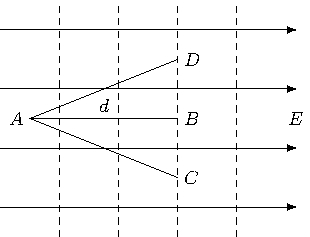
\includegraphics{fig/B/6-24.pdf}
	\caption{}\label{fig_B_6-24}
\end{figure}



我们再来研究场强和电势
差的数量关系.设图~\ref{fig_B_6-24} 中
$A$、$B$间的距离为$d$,电势差为
$U$,场强为$E$.把正电荷$q$从$A$
移到$B$时,电场力$qE$所做的功
$W=qEd$.利用电势差和功的
关系,这个功又可求得为$W=qU$.比较这两个式子,即可得
到
\[U=Ed\]
这就是说,\textit{在匀强电场中,沿场强方向的两点间的电势差等于
场强和这两点间距离的乘积}.

把上式改写成
\[E=\frac{U}{d} \]
这个等式说明,\textit{在匀强电场中,场强在数值上等于沿场强方向
每单位距离上降低的电势}.

由上式可以得到场强的另一个单位:伏特/米($\UVmA$).由于
\[1 \UVm = 1 \Uspace \frac{\UVA}{\UmA}=1\Uspace\frac{\UJCA}{\UmA}=1\Uspace\frac{\UNA\cdot \UmA}{\UCA\cdot \UmA}=1\Uspace\frac{\UNA}{\UCA} =1 \UNC  \]
所以场强的两个单位$\UVmA$和$\UNCA$是相等的.

\begin{example}
    图~\ref{fig_B_6-25} 中,金属圆板$A$、$B$相距3厘米.用电
压为60伏的电池组使它们带电,它们间的匀强电场的场强是
多大,方向如何?
\end{example}
\begin{figure}[htbp]
    \centering
    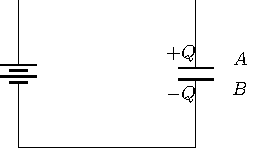
\includegraphics{fig/B/6-25.pdf}
    \caption{}\label{fig_B_6-25}
\end{figure}    

\begin{solution}
    金属板间的电势差就是电池组的电压.知道这个电势差
$U$后,可以用公式$E=U/d$计算出场强$E$:
\[E=\frac{U}{d}=\frac{60}{3\times 10^{-2}} \UVm=2\times 10^3 \UVm \]

$A$板带正电,$B$板带负电,所以场强方向是由$A$板指向$B$
板.
\end{solution}

\subsection*{练习八}

\begin{enumerate}
    \item 两块相距0.05米的带电平行板之间的电场是匀强
    电场,两板的电势差为$10^4$伏.求作用在两板之间的一个电
    子上的电场力.
    \item 平行的带电金属板$A$、$B$间是匀强电场(图~\ref{fig_B_6-26}),场
    强为$1.2\times10^8\UNC$.两板间的距离为5厘米,两板间的电
    势差有多大?电场中有两点$P_1$和$P_2$,$P_1$点离$A$板的距离是
    0.5厘米,$P_2$点离$B$板的距离也是0.5厘米.$P_1$和$P_2$两点间
    的电势差有多大?
\end{enumerate}

\begin{figure}[htbp]
    \centering
    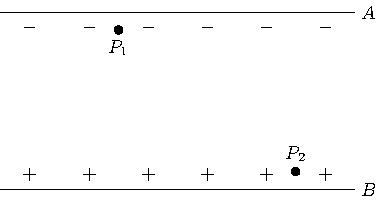
\includegraphics{fig/B/6-26.pdf}
    \caption{}\label{fig_B_6-26}
\end{figure}    

\section{带电粒子在电场中的运动}

带电粒子在电场中受到电场力的作用,产生加速度,速度
的大小和方向都可以发生变化.在现代科学实验和技术设备
中,常常根据这个道理,利用电场来改变或控制带电粒子的运
动.这种应用大致可以分成两种情况:一是利用电场来使带
电粒子加速,一是利用电场来使带电粒子偏转.

\subsection{带电粒子的加速}


如图~\ref{fig_B_6-27} 所示,在真空中有一对平行
金属板,接上电压为$U$的电池
组,在它们之间建立匀强电场.
设有一个正电荷$q$穿过正极板
上的小孔进入电场,在电场中
被加速,到达负极板时从负极
板上正对的小孔穿出.
正电荷穿出时的速度$v$是多大呢?正电荷$q$从正极板移到负极板,电
场力做的功$W=qU$.设$q$是在正极板处由静止开始运动,
到达负极板时它的动能为$\dfrac{1}{2}mv^2$.
根据动能定理得到$qU=\dfrac{1}{2}mv^2$.
由此就可求出电荷$q$到达负极板的速度
\[
v=\sqrt{2gU/m}
\]


\begin{figure}[htbp]
	\centering
	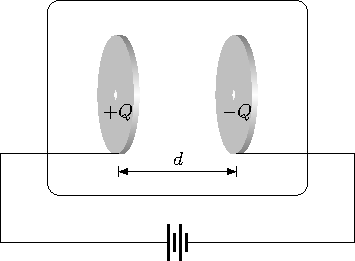
\includegraphics{fig/B/6-27.pdf}
	\caption{}\label{fig_B_6-27}
\end{figure}


带电粒子在匀强电场中的上述加速运动,跟物体在重力
场中的自由落体运动相似.不过,物体在重力场中受到的力
跟质量成正比,因此不同质量的物体具有相同的加速度;而带
电粒子在电场中受到的力跟电量成正比,质量相同的粒子可
以带有不同的电量,因而它们在电场中的加速度可以互不相
同.

上述用电压$U$来表达的计算速度的公式$v=\sqrt{2gU/m}$对
非匀强电场也适用.这是因为,不论在什么电场中,电荷$q$通
过电压$U$时,电场力对它做的功总等于$qU$,而对初速度为零
的带电粒子总是有$qU=\dfrac{1}{2}mv^2$
的关系.

\subsection{带电粒子的偏转}


要使以一定速度运动的带电粒子偏
转,可以有两个办法:一是利用磁场,这将在高中三年级再讨
论,一是利用电场.
利用电场使带电粒子偏转,人们通常用跟
带电粒子初速度方向垂直的匀强电场,这时带电粒子受到一
个跟原来运动方向垂直的电场力,因而发生偏转.
\begin{figure}[htbp]
    \centering
    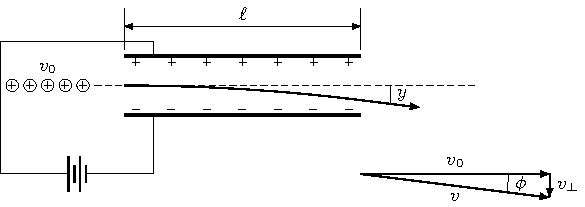
\includegraphics{fig/B/6-28.pdf}
    \caption{}\label{fig_B_6-28}
\end{figure}

如图~\ref{fig_B_6-28} 所示,真空中有一对平行金属板,接上电压为
$U$的电池组,在它们之间建立匀强电场,场强为$E=U/d$,
其中$d$为两板的距离.设有一些带正电荷$q$的粒子以初速度$v_0$进
入电场,$v_0$的方向跟$E$的方向垂直.带电粒子受到垂直于$v_0$
的侧向电场力$F=qE=qU/d$
的作用,它们在电场内的运动跟
物体在重力场中的平抛运动相似.现在我们来计算带电粒子
在电场中侧向移动的距离$y$.带电粒子在侧向电场力$F$作用
下,沿侧向做初速度为零的匀变速运动,所以$y=\dfrac{1}{2}at^2$.
由牛顿第二定律知道,
\[a=\frac{F}{m}=\frac{qU}{md} \]
带电粒子在电场内运动的时
间$t=\ell/v_0$.由此可得
\[y=\frac{qU}{2v^2_0 md}\ell^2 \]

带电粒子离开电场后,将在偏离原来运动方向某一角度
$\phi$的方向上做匀速直线运动.
研究带电粒子的偏转,这个偏
角$\phi$是特别重要的.现在来讨论$\phi$跟哪些因素有关.
带电粒子离开电场时得到一个垂直于初速度的侧向速度$v_{\bot}=at$.而
\[a=\frac{qU}{md},\qquad t=\frac{\ell}{v_0} \]
由此可得
\[v_{\bot}=at=\frac{qU\ell}{mdv_0} \]
带电粒子离开电场时的偏角$\phi$由下式确定:
\[\tan\phi=\frac{v_{\bot}}{v_0}=\frac{qU\ell}{mdv^2_0} \]
对于一定的带电粒子束,$m$、$q$、$v_0$都是确定了的,适当选择$U$、$d$、$\ell$,就可以使
$\phi$符合预定的要求.

\begin{example}
实验表明,赤热的金属丝可以发射电子.在图~\ref{fig_B_6-29} 
中,从赤热金属丝射出的电子流,经电场加速后进入偏
转电场.
已知加速电极间的电压是2500伏,偏转电极间的电
压是2.0伏,偏转电极长6.0厘米,相距0.2厘米.电子的质
量是$0.91\times10^{-30}$千克.求:
\begin{enumerate}
    \item 电子离开加速电场时的速度;
    \item 电子离开偏转电场时的侧向速度.
\end{enumerate}
\begin{figure}[htbp]
	\centering
	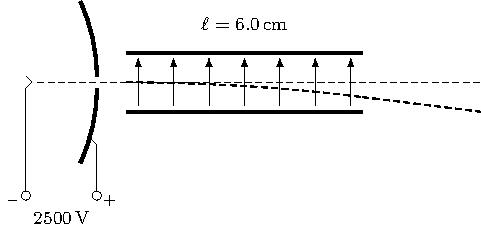
\includegraphics{fig/B/6-29.pdf}
	\caption{}\label{fig_B_6-29}
\end{figure}

\end{example}

\begin{solution}
\begin{enumerate}
\item 
经过2500伏的加速电场后,电子获得的动能
\[E_K=2500 \UeV =2500\times1.6\times10^{-19} \UJ=4.0\times10^{-16} \UJ \]
而$E_K=\dfrac{1}{2}mv^2$,所以
\[\begin{split}
	v=\sqrt{\frac{2E_K}{m}}&=\sqrt{\frac{2\times 4.0\times 10^{-18}}{0.91\times 10^{-30}}}\Ums\\
	&=3.0\times 10^7\Ums
\end{split} \]    

\item 
电子离开偏转电场时的侧向速度是
\[\begin{split}
	v_{\bot}&=\frac{qU\ell}{mdv}\\
	&=\frac{1.6\times10^{-19}\times2.0\times6.0\times10^{-2}}{0.91\times10^{-30}\times0.2\times10^{-2}\times3.0\times10^{7}} \Ums\\
	&=3.5\times 10^5\Ums
\end{split} \]    
\end{enumerate}
\end{solution}

\subsection*{练习九}
\begin{enumerate}
    \item 在真空中有一对平行金属板,相距6.2厘米,加上90
伏的电压.
两价的氧离子从静止出发被加速,从一板到达另
一板时,它的动能是多大?

这道题有几种解法?哪种解法比较简便?

\item 两价离子在90伏的电压下从静止加速后,测出它的
动量是$1.24\times10^{-21} \Ukgms$,这种离子的质量是多大?

\item 经1000伏加速电压加速后的电子,沿着与电场垂直
的方向进入匀强偏转电场,场强为5000$\UNC$.已知偏转电极长为6厘米.
求电子离开偏转电场时的速度.
\item 计算一下本节例题中的电子离开偏转电场时侧向移
动的距离.
\item 图~\ref{fig_B_6-30} 所示的实验装置可以用来验证电场对带电
粒子的加速作用只跟电压有关.左边的非匀强电场使电子加
速,右边的匀强电场使电子减速.
设非匀强电场的电压为$U$,
匀强电场的电压为$U'$.实验结
果是:只要$U'<U$,电流计的指
针就偏转;只要$U'>U$,电流计
的指针就不偏转.你从这个实
验结果可以得出什么结论?
\begin{figure}[htbp]
    \centering
    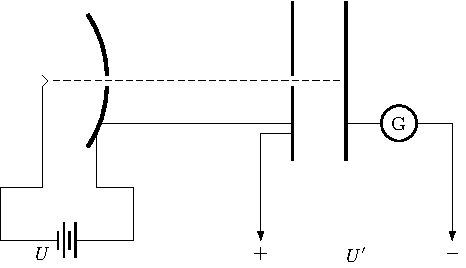
\includegraphics{fig/B/6-30.pdf}
    \caption{}\label{fig_B_6-30}
\end{figure}
\end{enumerate}

\section{基本电荷的测定:密立根实验}

电子和质子带有等量异种电荷.
实验指出,它们所带的
电量都是$e=1.60\times10^{-19}$库.实验还指出,所有电量或者等
于电子或质子的电量,或者是它们的电量的整数倍,因此,人
们把$1.60\times10^{-19}$库的电量叫做基本电荷.

历史上对电子电荷的测定进行了一系列实验.
电子电荷的精确数值最早是美国科学家密立根($1868 \sim 1953$)于1917
年用实验测得的.密立根实验是物理学的经典实验之一,下
面从原理上介绍一下这个实验的最简单的方法.


密立根实验仪器示意图如~\ref{fig_B_6-31a} 所示.$A$、$B$是两块平
行放置的水平金属板,把它们与电源相接,使$A$板带正电,$B$
板带负电.油滴从喷雾器喷出,经过上板当中的小孔,落到
$A$、$B$之间的匀强电场中.
油滴出来时由于摩擦而带电,假如
油滴带负电,它要受到方向向上的电场力$F$作用.油滴还受到
重力$mg$的作用.调节两个板间的电势差,可使带有电量为
$q$的某个油滴所受的电场力$Eq$恰好和重力$mg$平衡(图~\ref{fig_B_6-31b}),于是油滴悬浮在电场中保持不动.在这种情况下,$Eq=
mg$.根据这个式子可以求出电量$q$:
\[q=\frac{mg}{E}=\frac{mgd}{U}  \]
上式中$U$是两板间的电势差,$d$是两板的距离,它们都可以直
接测得.但是油滴太小,$m$很难直接测量.密立根设法用实验
测出油滴的半径$r$,然后用体积公式$V=\dfrac{4}{3}\pi r^3$
算出油滴的体积,再用油滴的体积乘以油滴的密度算出油滴的质量$m$.这
样,用上式即可得出油滴所带电量$q$.

\begin{figure}[htbp]
	\centering
	\begin{subfigure}{0.6\linewidth}
		\centering
		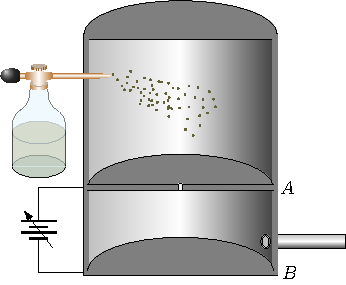
\includegraphics{fig/B/6-31a.pdf}
		\caption{}\label{fig_B_6-31a}
	\end{subfigure}
	\hfil
	\begin{subfigure}{0.3\linewidth}
		\centering
		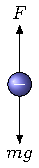
\includegraphics{fig/B/6-31b.pdf}
		\caption{}\label{fig_B_6-31b}
	\end{subfigure}
	\caption{}\label{fig_B_6-31}
\end{figure}



密立根测定了数千个带电油滴的电量,他对测得的数据
进行分析研究,发现这些电量都等于某个最小电荷的整数倍,
这个最小电荷就是电子或质子所带的电量$e$.在密立根实验
之后,人们还做了许多其他实验,进一步精确地测定电子的电量.
现在测得的基本电荷的精确值是
\[e=1.6021892\times10^{-19} \UC \]
通常可取作
\[e=1.60\times10^{-19} \UC \]

基本电荷是物理基本常数之一,测定它在理论上和实际
上都有重大意义.

密立根实验进一步证实了电子的存在,揭示了电荷的非
连续性,即自然界中的任何电量都只能是某一基本单位的整
数倍,而不能连续变化\footnote{近年来在高能物理的研究中提出了一个设想,认为质子、中子
等粒子是由更基本的层子(又叫夸克)组成的,层子所带电量是基本电
荷的$1/3$或$2/3$.但是,人们一直还没有在实验中观察到层子.}.

\section{电容器~~电容}
\subsection{电容器}
任何两个彼此绝缘而又互相靠近的导体,都可
以看成是一个电容器.这两个导体就是电容器的两个极.
两块正对的平行金属板,它们相隔很近而且彼此绝缘,就组成一
个最简单的电容器,叫做平行板电容器.

使电容器带电叫做充电.充电时总是使电容器的一个导
体带正电,另一个导体带等量的负电.
每个导体所带电量的
绝对值,叫做电容器所带的电量.把平行板电容器的一个极
板接电池组的正极,另一个极板接电池组的负极,两个极板就
分别带上等量的异种电荷.

使充电后的电容器失去电荷叫做放电.
用一根导线把电
容器的两极接通,两极上的电荷互相中和,电容器就不带电
了.

电容器是电气设备中的重要元件之一,在电子技术和电
工技术中有很重要的应用.

\subsection{电容}
电容器带电的时候,它的两极之间产生电势差.实
验证明,对任何一个电容器来说,两极间的电势差都随所带电
量的增加而增加,而且电量跟电势差成正比,它们的比值是一个恒量.
不同的电容器,这个比值一般是不同的.可见,这个
比值表征了电容器的特性.\textit{电容器所带的电量跟它的两极间
的电势差的比值,叫做电容器的\textbf{电容}}.如果用$Q$表示电容器
所带的电量,用$U$表示它的两极间的电势差,用$C$表示它的电
容,那么,
\[C=\frac{Q}{U} \]

电容器带电的情形可以用直筒容器装水的情形来比喻.
直筒容器装水后水的深度总跟装的水量成正比,水量和水的
深度的比值是一个恒量.不同的直筒容器,这个比值一般是
不相同的.
这个比值越大,即水面升高单位高度所需的水量
越大,表示容器的容量越大.

在国际单位制里,电容的单位是法拉,简称法,国际符号
是$\UFA$.一个电容器,如果带1库的电量时两极间的电势差是
1伏,这个电容器的电容就是1法.
\[1 \UF=1\UCV \]

法拉这个单位太大,实际上常用较小的单位:微法($\UuFA$)
和皮法($\UpFA$).它们间的换算关系是:
\[1 \UF=10^6\UuF=10^{12} \UpF \]

无线电收音机里常用的电容器,电容从几个皮法到几十
个微法的都有.

\subsection{平行板电容器的电容}


现在我们来研究平行板电容器的
电容跟哪些因素有关.

如图~\ref{fig_B_6-32} 所示,让平行板电容器带电后,用静电计\footnote{静电计是在验电器的基础上制成的,用来测量导体间的电势
差.使用时把它的金属球跟一个导体连接,把它的金属外壳跟另一个
导体连接或同时接地,从指针的偏转角度就可以知道两个导体间的电
势差.}来
测量两极板$A$、$B$间的电势差.
不改变$A$、$B$两极板所带的电
量,只改变两极板间的距离,可以看到,距离越大,静电计指出
的电势差越大.这表示平行板电容器的电容随两板距离的增
大而减小.

\begin{figure}[htbp]
    \centering
    \begin{minipage}[t]{0.48\textwidth}
        \centering
        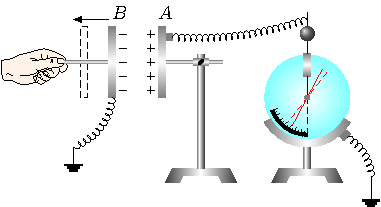
\includegraphics{fig/B/6-32.pdf}
        \caption{}\label{fig_B_6-32}
    \end{minipage}
    \begin{minipage}[t]{0.48\textwidth}
        \centering
        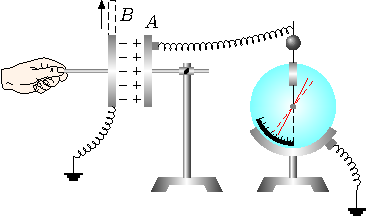
\includegraphics{fig/B/6-33.pdf}
        \caption{}\label{fig_B_6-33}
    \end{minipage}
\end{figure}

    如图~\ref{fig_B_6-33} 所示,不改变两极板所带电量和它们的距离,
    只改变两极板的正对面积,可以看到,正对面积越小,静电计
    指出的电势差越大.这表示平行板电容器的电容随两极板的
    正对面积的减小而减小.
   

    如图~\ref{fig_B_6-34} 所示,保持两极板所带电量、它们的距离、它们
    的正对面积都不改变,而在极板间插入电介质,可以看到,静
    电计指出的电势差减小.这表示平行板电容器的电容由于插
    入电介质而增大.
	
	 \begin{figure}[htbp]
		\centering
		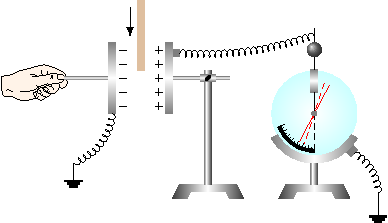
\includegraphics{fig/B/6-34.pdf}
		\caption{}\label{fig_B_6-34}
	\end{figure}



    由于我们的知识不足,现在还不能从理论上进一步讨论
    上面的实验结果.
    可以指出:对于一个平行板电容器,如果两
    板的正对面积为$S$,两板的距离为$d$,两板间充满介电常数为
    $\varepsilon$的电介质,那么,它的电容可以用下式来表示.
\[C=\frac{\varepsilon S}{4\pi kd} \]
式中$S$用$\UmqA$作单位,$d$用$\UmA$作单位,静电力恒量$k=9\times 10^9 \UNmqCq$,算出的$C$以法为单位.
可以看出,\textit{平行板电容器
的电容,跟介电常数成正比,跟正对面积成正比,跟极板的距
离成反比}.这跟上面的实验结果是一致的.

一般说来,电容器的电容是由两个导体的大小和形状、两
个导体的相对位置以及它们间的电介质定的.

\subsection{常用电容器}

懂得了决定电容大小的因素,就可以利用
这些知识来改变电容器的电容.实际上,人们正是这样制成
各种电容器,来满足不同需要的.从构造上看,常用的电容器
可分为固定电容器和可变电容器两类.

固定电容器的电容是固定不变的,由于所用的电介质不
同,又可分为纸介电容器、云母电容器、瓷介电容器、电解电容器等.
下面我们说明一下纸介电容器和电解电容器.

纸介电容器是在两层锡箔或铝箔中间夹以在石蜡中浸过
的纸,一起卷成圆柱体而制成的(图~\ref{fig_B_6-35}).纸浸过石蜡后,
可避免潮气侵入,使绝缘能力大大增强.改变锡箔或铝箔
的面积,可以制成电容大小不同的纸介电容器.这种电容器
的特点是容易制造出电容较大的电容器,而且价格较低.
\begin{figure}[htbp]
    \centering
    \begin{minipage}[t]{0.35\textwidth}
        \centering
        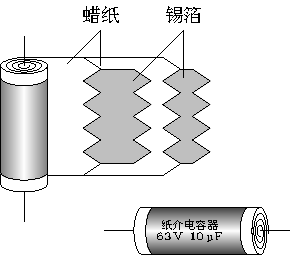
\includegraphics{fig/B/6-35.pdf}
        \caption{纸介电容器}\label{fig_B_6-35}
    \end{minipage}
    \begin{minipage}[t]{0.3\textwidth}
        \centering
        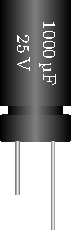
\includegraphics{fig/B/6-36.pdf}
        \caption{电解电容器}\label{fig_B_6-36}
    \end{minipage}
    \begin{minipage}[t]{0.3\textwidth}
    	\centering
    	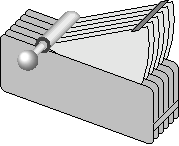
\includegraphics{fig/B/6-37.pdf}
    	\caption{可变电容器}\label{fig_B_6-37}
    \end{minipage}
\end{figure}

电解电容器外形如图~\ref{fig_B_6-36} 所示.
这种电容器的极性是
固定的,使用时正负极不能接反,并且不能接在交流电路中,
否则它将不能工作,这是它跟其他电容器不同的地方.
电解电容器是利用电解现象制成的,它的原理将在后面第\ref{chapter-conductivity-of-matter}章中给予说明.


可变电容器的电容是可以改变的,它由两组铝片组成(图~\ref{fig_B_6-37}),
固定不动的一组铝片叫定片,可以转动的一组铝片叫
动片.
定片和动片之间的电介质,通常就用空气.
转动动片,两组铝片的正对面积发生变化,电容就随着改变.

此外,还有半可变电容器,能微小地调整两极片间的距离
或改变它们的正对面积,使电容发生微小改变.图~\ref{fig_B_6-38} 是电
路图中常用的几种电容器的符号.

\begin{figure}[htbp]
    \centering
    \begin{subfigure}{0.2\linewidth}
        \centering
        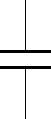
\includegraphics{fig/B/6-38a.pdf}
        \caption{}\label{fig_B_6-38a}
    \end{subfigure}
    \hfil
    \begin{subfigure}{0.2\linewidth}
        \centering
        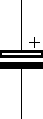
\includegraphics{fig/B/6-38b.pdf}
        \caption{}\label{fig_B_6-38b}
    \end{subfigure}
    \hfil
    \begin{subfigure}{0.2\linewidth}
        \centering
        \includegraphics{fig/B/6-38c.pdf}
        \caption{}\label{fig_B_6-38c}
    \end{subfigure}
    \hfil
    \begin{subfigure}{0.2\linewidth}
        \centering
        \includegraphics{fig/B/6-38d.pdf}
        \caption{}\label{fig_B_6-38d}
    \end{subfigure}
    \caption{从左到右依次是:固定电容器,电解电容器,可
    变电容器,半可变电容器.}\label{fig_B_6-38}
\end{figure}

加在电容器两极上的电压不能超过某一限度.超过这个
限度,电介质将被击穿,电容器于是损坏,这个极限电压叫做击穿电压.
电容器工作时的电压应低于击穿电压.
电容器上一般都标明了电容和额定电压的数值.电容器的额定电压是
指电容器长期工作所能承受的电压,它比击穿电压要低.

\subsection*{练习十}
\begin{enumerate}
    \item 电容器带电后电势差增大的情形,跟物体吸收热量后温度升高的情形也很相似.
    试对这两种现象作一比较.
    \item 一个由圆板制成的平行板电容器,圆板的半径为3.0
厘米,两板的距离为2.0毫米,中间充满介电常数为6.0的电
介质.
这个电容器的电容是多少?
\item 一个电容器的电容是$1.5\times10^{-2}$微法,把它的两个极
板接在90伏的电源上,求每个极板上的电量.
\item 有一个电容器,在带了电量$Q$以后,两导体间的电势差是$U$.
如果使它带的电量增加$4.0\times10^{-8}$库,两导体间的电势差就增大20伏.
这个电容器的电容是多少微法?


\item 如图~\ref{fig_B_6-39} 所示,闭合
电键$K$使平行板电容器$C$充
电,然后断开电键.
当增大电容
器两板间的距离时,下述各量
是否改变,怎样改变?
\begin{enumerate}
    \item 电容器所带电量;
    \item 电容器的电容;
    \item 电容器两板间的电势差.
\end{enumerate}

\begin{figure}[htbp]
	\centering
	\includegraphics{fig/B/6-39.pdf}
	\caption{}\label{fig_B_6-39}
\end{figure}

\item 在上题中,充电后如果保持电键$K$闭合,那么,增大
电容器两板间的距离时,下述各量是否改变,怎样改变?
\begin{enumerate}
    \item 电容器两板间的电势差;
    \item 电容器的电容;
    \item 电容器所带的电量.
\end{enumerate}
\end{enumerate}

\section{电容器的连接}
实际使用电容器时,有时会遇到电容器的电容不够或耐
压能力不够,这就需要把几个电容器连接起来使用,连接的基
本方法有串联和并联两种.
\subsection{电容器的串联}

把几个电容器的极板首尾相接,连成一
串,这就是电容器的串联.
图~\ref{fig_B_6-40} 是三个电容器的串联.
接上电压为$U$的电源后,两端极分别带电$+Q$和$-Q$.由于静
电感应,中间各极所带的电量也等于$+Q$或$-Q$,所以串联时
每个电容器带的电量都是$Q$.如果各个电容器的电容分别为
$C_1$、$C_2$、$C_3$,电压分别为$U_1$、$U_2$、$U_3$,那么,
\[ U_1=\frac{Q}{C_1},\qquad U_2=\frac{Q}{C_2},\qquad U_3=\frac{Q}{C_3}\]
总电压$U$等于各个电容器上的电压之和,所以,
\[U=U_1+U_2+U_3=Q\qty(\frac{1}{C_1}+\frac{1}{C_2}+\frac{1}{C_3})\]
设串联电容器的总电容为$C$,则$U=Q/C$,所以
\[\frac{1}{C}=\frac{1}{C_1}+\frac{1}{C_2}+\frac{1}{C_3}\]
这就是说,\textit{串联电容器的总电容的倒数等于各个电容器的电
容的倒数之和}.电容器串联之后,相当于增大了两极的距离,
因此总电容小于每个电容器的电容.

\begin{figure}[htbp]
    \centering
    \begin{minipage}[t]{0.45\linewidth}
    	\centering
    	\includegraphics{fig/B/6-40.pdf}
    	\caption{电容器的串联}\label{fig_B_6-40}
    \end{minipage}
    \hfil
    \begin{minipage}[t]{0.45\linewidth}
    	\centering
    	\includegraphics{fig/B/6-41.pdf}
    	\caption{电容器的并联}\label{fig_B_6-41}
    \end{minipage}
\end{figure}



\subsection{电容器的并联} 


把几个电容器的正极连在一起,负极也
连在一起,这就是电容器的并联.图~\ref{fig_B_6-41} 是三个电容器的并
联.接上电压为$U$的电源后,每个电容器的电压都是$U$.如
果各个电容器的电容分别为$C_1$、$C_2$、$C_3$,所带电量分别为$Q_1$、$Q_2$、$Q_3$,那么,
\[Q_1=C_1U,\qquad Q_2=C_2U,\qquad Q_3=C_3U\]
电容器组贮存的总电量$Q$等于各个电容器所带电量之和,
所以,
\[Q=Q_1+Q_2+Q_3=(C_1+C_2+C_3)U\]
设并联电容器的总电容为$C$,则$Q=CU$,所以,
\[C=C_1+C_2+C_3\]
这就是说,\textit{并联电容器的总电容等于各个电容器的电容之和}.
电容器并联之后,相当于增大了两极的面积,因此总电容大于
每个电容器的电容.

电容器串联后,电容减小了,但耐压能力提高了,所以要
承受较高的电压,可以把电容器串联起来;电容器并联后,电
容增大了,耐压能力没有提高,所以在需要大电容时,可把
电容器并联起来.

\begin{example}
电容器$A$的电容为10微法,充电后电压为30伏.
电容器$B$的电容为20微法,充电后电压为15伏.
把它们的正极连在一起,负极连在一起后,它们的电压是多少?
\end{example}


\begin{solution}
连接前电容器$A$的电量为
\[Q_1=C_1U_1=10\times10^{-8}\times30 \UC =3.0\times10^{-4} \UC \]
连接前电容器$B$的电量为
\[Q_2=C_2U_2=20\times10^{-8}\times 15 \UC =3.0\times10^{-4} \UC \]
它们的总电量为
\[Q=Q_1+Q_2=6.0\times10^{-4} \UC \]
这个总电量并不会因为连接而改变.
连接后的总电容为
\[C=C_1+C_2=3.0\times10^{-5} \UF \]
连接后的共同电压为
\[U=\frac{Q}{C}=\frac{6.0\times10^{-4}}{3.0\times10^{-5}} \UV =20 \UV \]
\end{solution}

有兴趣的同学还可以进一步计算连接后每个电容器的电
量,看看电荷是从哪个电容器流到另一个电容器的.

\subsection*{练习十一}

\begin{enumerate}
\item 两个相同的电容器,标有“100皮法、600伏”,串联后接到900伏的电路上.
每个电容器带多少电?加在每个电容器
上的电压是多少?电容器是否会击穿?
\item 把“100皮法、600伏”和“300皮法、300伏”的电容器
串联后接到900伏的电路上,这样连接是否合适?为什么?
\item 平行板电容器的正对面积为$S$,
两板距离为$\ell$,电介质是真空.如果在两
板之间插入一厚度为$d$的金属板(图~\ref{fig_B_6-42}),试证明它的电容为
\[C=\frac{S}{4\pi k(\ell-d)}\]
\begin{figure}[htbp]
    \centering
    \includegraphics{fig/B/6-42.pdf}
    \caption{}\label{fig_B_6-42}
\end{figure}
\item 电容分别为20微法和50微法的
两个电容器并联后,接在电压为100伏的
电路上,它们共带多少电?
\item 电容为 3000 皮法的电容器带电
$1.8\times10^{-6}$库后,撤去电源,再把它跟电容为1500皮法的电容器并联.
求每个电容器所带电量.
\end{enumerate}

\section{静电的防止和应用}
静电现象是一种常见的自然现象.
用塑料梳子梳头发,梳子会吸引头发,有时还会听到响声.
脱下尼龙衣服时,有时
也会听到响声,在黑暗中还能看到火花.
静电一般是由摩擦
产生的.当两个物体相互摩擦时,它们带上了异种电荷,它们
之间就产生了电势差.
电荷积累到一定数量,电势差达到一
定数值时,就如同电容器被击穿一样,带电物体之间发生放电
现象(见第\ref{chapter-conductivity-of-matter}章第\ref{sec_B-8-6}节),我们就可能看到火花,听到响声.

静电会给人们带来麻烦和危害.
在印刷工业中,纸张上带的静电吸引空气中的尘埃或带颜色的微粒,会使印刷质量下降.
在合成纤维的生产中,由于静电吸引空气中的尘埃,会
使产品质量下降.
在制药生产中,由于静电吸引尘埃,会使药
品达不到标准的纯度.
静电对现代高精密度、高灵敏度的电
子设备颇有影响.带静电很多的人甚至可以使那些灵敏、脆
弱、小巧玲珑的电子器件被击穿,因而毁坏一部电子仪器.
在家庭中,带静电很多的人从电视机旁走过,会给电视的图像和
声音带来干扰.

静电的最大危害是有可能因静电火花点燃某些易燃物
质,而引起爆炸.石油在管道中流动时,油类从管道口或管道
裂缝高速喷出时,含有煤尘的空气在风管中流动时,向油槽内
灌油时,都会因摩擦而产生静电.
一旦电荷积累相当多,达到
相当高的电压(可以达到上千伏甚至上万伏),就会发生放电而引起爆炸.
静电现象是很普遍的.在外科手术台上也出现
过静电火花使乙醚爆炸的事件.

怎样防止静电的危害呢?最简单而又最可靠的办法是用
导线把设备接地,这样可以把电荷引入大地,避免静电积累.
大型油罐要有很多条接地线.
油罐车的尾部拖一条铁链,它就
是车的接地线.
调节空气的湿度也是防止静电危害的有效方
法.湿度增大时,电荷随时放出,无法积累,静电危险也就消除了.
潮湿的天气里不容易做好静电实验,也是这个道理.

跟其他物理现象一样,静电现象也可以被人们利用.
随着科学技术的发展,静电技术已经有了长足的进步.

在电场中,带电粒子受到电力的作用,向着电极运动,最
后会被吸在电极上.
利用这个道理可以除去或收集空气中的尘粒.
设法使空气中的尘粒带电,在电力作用下尘粒到达电
极而被收集起来,这就是静电除尘.
制造各种精密的元件或
仪器,对空气的净化程度要求很高,空气中的微粒多,会严重影响产品的质量.
利静电除尘可以有效地提高空气的净化
程度.静电除尘还可用于粉尘较多的场所,除去空气中对人
们有害的微粒.
静电除尘也可用来回收物资,如回收水泥粉尘.

依据相同的道理,可以利用静电方法在物体上喷涂液体
或固体涂料.
达就是静电喷涂.
例如设法使油漆的微粒带电,
在电力作用下,油漆微粒飞向作为电极的工件,并沉积在工
件表面上,完成油漆工件的任务.
使塑料粉末带电,用静喷
涂可以在工件的表面涂上一层均匀光滑且具有高绝缘性能的
塑料涂层.
静电喷涂已广泛地用于对自行车、汽车、电气产品
以及家具进行喷涂.
利用类似的方法,使绒毛带电,可以把绒
毛植在涂有粘着剂的纺织物上,形成象刺绣似的纺织品,这就
是静电植绒.在喷雾器和植物(例如苹果树)之间建立起静电
场,可以使农药的液滴或粉粒准确地飞向目标,有效地喷撒
农药.

不同种类的粒子,它们在静电场中表现的行为不同,利用
这个道理我们可以把它们区分开来,这就是静电分选.
小麦等细长形状的种子,在强电场中,它们自身的方向会按照电力
线的方向排列起来,不同的种子使它们按电力线方向排列起
来的场强不同,这样就可以对种子进行分选.
静电分选有不
同的分选方式,利用不同的分选方式,可以除去米糠,可以分
选茶叶,可以分选矿石和煤炭,可以分选塑料被覆线的铜芯和
塑料包皮,还可以对城市垃圾进行处理回收.

静电技术还用于摄影、复印等方面.
静电复印现在已经
有了广泛的应用,它可以把报纸、书刊、文件等印刷品以及工
程蓝图、手写稿等,直接复印在白纸上,大大提高了复制的
速度.

静电技术应用很广,发展很快,有许多课题在等待着人们
去探索,去研究.

\section*{复习题}
\begin{enumerate}
\item 电荷守恒定律的内容是什么?
\item 库仑定律的内容是什么?写出在真空中和电介质中
库仑定律的公式.
静电力恒量的数值是多大?
\item 什么是电场强度?电场中某点的场强在数值上等于
什么?方向是怎样规定的?写出场强的定义式和点电荷在真空
中和在充满电介质空间里各点场强的计算式.
\item 电荷在电场中某点的电势能在数值上等于什么?什
么是电势?电场中某点的电势在数值上等于什么?
\item 什么是电势差?知道了电场中两点的电势差,怎样计
算在这两点间移动电荷时电场力所做的功?在匀强电场中电
势差跟电场强度有什么关系?
\item 用电力线和等势面可以形象地表示电场.
知道了某
一电场的电力线或等势面的分布情况,能不能形象地表示场
强的大小和方向?能不能形象地表示电势的高低?是怎样表
示的?
\item 处于静电平衡状态的导体,内部的场强是怎样的?表
面上任一点场强的方向是怎样的?各点的电势是怎样的?电
荷是怎样分布的?
\item 说明用电场使带电粒子加速和偏转的原理.
\item 说明密立根实验的原理,基本电荷的电量是多大?
\item 什么是电容器的电容?平行板电容器的电容跟哪些
因素有关?各是什么关系?写出平行板电容器电容的公式.
\item 串联电容器的总电容等于么?并联电容器的总电
容等于什么?在什么情况下,需要把电容器串联起来?在什么
情况下,需要把电容器并联起来?
\end{enumerate}

\section*{习题}
\begin{enumerate}
\item 有一个绝缘的金属筒,上面开个小孔,通过小孔放入
一个悬挂在丝线上的带正电的小球.
在下列各种情况里,金
属筒外壁各带什么电荷?
\begin{enumerate}
\item 小球跟筒的内壁不接触;
\item 小球跟筒的内壁接触;
\item 小球跟筒的内壁不接触,但用手指接
触一下金属筒,然后移开手指,再把小球移出筒外.
\end{enumerate}

\item 有两个带电小球,电量分别为$+Q$和$+9Q$,在真空
中相距0.4米.如果引进第三个带电小球,正好使三个小球都
处于平衡状态,第三个小球带的是哪种电荷?应放在什么地
方?电量是$Q$的几倍.
\item 如图~\ref{fig_B_6-43} 所示,有两
个挂在丝线上的小球,带有等
量的同种电荷,由于电荷彼此
推斥,丝线都偏离竖直线$\theta$角.
已知两小球的质量都为$m$,两丝线长都为$\ell$,求每个小球上所带的电量.

\begin{figure}[htbp]
    \centering
    \begin{minipage}[t]{0.48\textwidth}
        \centering
        \includegraphics{fig/B/6-43.pdf}
        \caption{}\label{fig_B_6-43}
    \end{minipage}
    \begin{minipage}[t]{0.48\textwidth}
        \centering
        \includegraphics{fig/B/6-44.pdf}
        \caption{}\label{fig_B_6-44}
    \end{minipage}
\end{figure}



\item 在氢原子中,可以认为核外电子沿圆形轨道绕原子
核(质子)旋转,轨道半径为$5.3\times10^{-11}$米.
电子沿轨道运动
的动能是多大?
\item 下面一些说法哪个正确,哪个错误?说明理由.
\begin{enumerate}
\item 在匀强电场中电势处处相等.
\item 沿着电力线的方向场强越来越小.
\item 正电荷在电场中只能由电势高的地方向电势低的地
方跑.
\item 电荷在电场中只能向着电势能低的地方跑.
\item 初速度为零的电荷在电场中一定向着电势能低的地
方跑.
\end{enumerate}
\item 两块靠近的平行金属板,在两板之间为真空时,使它
们分别带上等量的异种电荷.
保持两板带的电量不变,如果
将两板间的距离减小为原来的1/3,两板间的电势差是原来
的多少倍?两板间匀强电场的场强是原来的多少倍?
\item 上题中,保持两板带的电量不变,而在两板间充满介
电常数为$\varepsilon$的电介质,两板间的电势差和匀强电场的场强将
如何改变?
\item 有一个电容器,电容是$1.5\times10^{-4}$微法,把它的两板
分别跟直流电源的正负极相连,使两板分别带电$6\times10^{-8}$库
和$-6\times10^{-8}$库.
如果两板的距离为1毫米,电容器两板间的
电场强度是多大?
\item 两个相当大的平行金属板相
距10厘米.
两板分别跟电池组的正
负极连接,两板间的一个小电荷受到
的电场力为$3\times10^{-4}$牛.
现在把两板
的距离增加到15厘米,如果连接的电
池组不变,小电荷受到的力变为多大?
如果在增大两板距离时把所连电池组
换成3倍电压的电池组,小电荷受到
的力又将变为多大?



\item 如图~\ref{fig_B_6-44},质量为$4.5\times
10^{-3}$千克的带电小球用2.0米长的线
悬挂在带等量异种电荷的平行板之
间,平衡时小球偏离竖直位置 2.0厘
米.
\begin{enumerate}
    \item 小球受到的电场力是多大?
    \item 如果两板间的电压是$1.5\times10^4$伏,两板的距离是10厘米,
那么,小球带有多少个多余的电子?
\end{enumerate}
    

\item 在图~\ref{fig_B_6-29} 中,先让一束电子,后让一束氢核通过偏转电场.
设:
\begin{enumerate}
	\item
	电子和氢核的初速度相同;
	\item
	电子和氢核原来的动能相同;
\end{enumerate}
试分别求出两种情况下电子的偏角$\phi_e$和氢核
的偏角$\phi_H$的正切之比.



\item 图~\ref{fig_B_6-45} 是用来使带正电的粒子加速和偏转的装置.
如果让氢和氦进入并电离,我们将得到一价氢离子、一价
氦离子和二价氦离子的混合物.它们经过同一电场加速后,
在同一电场里偏转,它们是否会分为三股,从而到达荧光屏后
产生三个亮点?回答中要说明理由.

\begin{figure}[htbp]
	\centering
	\includegraphics{fig/B/6-45.pdf}
	\caption{}\label{fig_B_6-45}
\end{figure}


\end{enumerate}




